% http://www.idsc.ethz.ch/education/theses-semester-projects.html
% IDSC LaTeX Thesis Template
% 
% Author(s):	Eric Müller
% 				Institute for Dynamic Systems and Control
% 				Swiss Federal Institute of Technology (ETH) Zurich
% 
% Created:		2004/04/02  (Eric Mueller)
% 
% Notes: Has been tested on Windows 7 + MikTeX + TeXnicCenter
%
% Revisions: 	2009/05/29  (Soren Ebbesen)
% 				    2011/03/22	(Soren Ebbesen)
%             2013/03/08	(Soren Ebbesen)
%             2014/03/13	(Soren Ebbesen)
% ______________________________________________________________________________
\documentclass[11pt,twoside,a4paper,fleqn]{report}

% specifies to what depth sections shall be enumerated
\setcounter{secnumdepth}{5}
%changes the white space padding below figures
%5pt stands for the padding between float elements (figures), the plus 2pt stands for a fixed 2pt (minus would mean optional)
\setlength{\intextsep}{5pt plus 2pt}   % default value 12pt plus 2pt minus 2pt

\usepackage[english,mt]{ethidsc} % Special IDSC styles and commands      	
								 % {german}/english: language of headings, etc.
								 % {st}/bt/mt: {semester}/bachelor/master thesis
%Footnotes
\renewcommand{\thefootnote}{\arabic{footnote}}
% for image positioning
\usepackage[export]{adjustbox}
\usepackage{wrapfig}
\usepackage{graphicx}
% defining the bibliography settings
\usepackage[backend=biber, citestyle=authoryear]{biblatex}
\addbibresource{library.bib}

% placing figures next to each other with subfigures
\usepackage{subcaption}
\usepackage{caption}
\newcommand{\source}[1]{\caption*{Source: {#1}} }
% for displaying code snipplets
\usepackage{listings}
\usepackage{enumitem}
\usepackage{amsmath}
\usepackage{mathtools}
% change h and vline thinkness
\usepackage{makecell}
\usepackage{array}
\newcolumntype{?}{!{\vrule width 1pt}}
							
% Page header (don't change)____________________________________________________
\setlength{\parindent}{0em}                 % Disable parindent
\rhead[\nouppercase{\rightmark}]{\thepage}  % Special headings
\lhead[\thepage]{\nouppercase{\leftmark}}   % Special headings
\cfoot{}                                    % Special headings


% Title page (please fill in)___________________________________________________
%\title{Using a classification model trained on text and image-data to predict nature-based recreation activities in geo-referenced social media content}

\title{Using a model trained on text and image-data to predict leisure activities in social media content.}


\studentA{Maximilian Hartmann (13-061-619)}
\ethidA{13-061-619}
\semesterA{9}
\emailA{hartmanm@student-net.ethz.ch}

%\studentB{Second Student}
%\ethidB{12-345-678}
%\semesterB{9}
%\emailB{second@student.ethz.ch}

\supervision{Dr. Marcel Hunziker (ETH and WSL)\\ Dr. Flurina Wartmann (WSL)\\ Prof. Dr. Ross Purves (UZH)\\ Dr. Rahul Deb Das (UZH)}

\date{Submission: 15\textsuperscript{th} of April 2019}

%\identification{IDSC-XX-YY-ZZ} 		% Project identifier

\infopage
\declaration

% Begin document___________________________________________________________

\begin{document}

\maketitle 							% Create title page


% Preamble______________________________________________________________________

\pagenumbering{roman} 				% Begin roman page numbering (i,ii,...)

%---------------------------------------------------------------------------
% Preface
% asterisk signals a title without numbering
%\chapter*{Preface}
%\

%Blah blah \dots

% \clearpage
%---------------------------------------------------------------------------
% Abstract

%\chapter*{Zusammenfassung}
% \addcontentsline{toc}{chapter}{Zusammenfassung}

%Bla bla \dots

\cleardoublepage

\chapter*{Abstract}
 \addcontentsline{toc}{chapter}{Abstract}
 XXXstart with a questions maybeXXX
 Can social media data function as a supplement to traditional survey data to evaluate spatial distributions of nature-based recreation activities?

Blah blah \dots

\cleardoublepage

\chapter*{Acknowledgements} \label{acknowledgements}
  \addcontentsline{toc}{chapter}{Acknowledgements}
I would like to express my very great appreciation to all my supervisors, friends and institutions that helped me during the course of this thesis. First of all I want to thank ETH for providing me with the infrastructure, research literature and needed resources that allowed the start and completion of this thesis.\\
Personally I want to sincerely thank Dr. Marcel Hunziker for approving my master thesis proposal that originated from a term paper of the 'Advanced Landscape Research' lecture which he also supervised. \\
I would like to offer my special thanks to Dr. Flurina Wartmann from the WSL who was my primary contact throughout the entire thesis and who assisted me in setting up the ground truthing as well as in various administrative concerns. \\
Prof. Dr. Ross Purves and Dr. Rahul Deb Das from the geocomputation unit of the University of Zurich provided me with expert knowledge in all programming related issues for which I am deeply grateful.\\
\newline
Additionally, I would like to thank the spatial planing department of the Canton of Zug - especially Martina Brennecke and Alexander Gnos. Former for her personal assistance and insight on relevant projects in the research area and latter for his provision of needed geo-data in the form of shapefiles. My special thanks are extended to the staff of the company Zugerbergbahn, particularly to Christoph Sidler for providing me with passenger numbers of their mountain railway. \\
\newline
I cannot thank my sister Florence enough for conducting the entire 'passive observation' - an essential part of the ground truthing. This part would not have been possible without her. And finally I want to thank and mention my friends Achilleas Lehmann and Christopher O'Bryan who proofread my thesis and gave constructive feedback that lead to this final version of my thesis.

\cleardoublepage
%---------------------------------------------------------------------------
% Table of contents

 \setcounter{tocdepth}{2}
 \tableofcontents
 \listoftables\addcontentsline{toc}{chapter}{List of Tables}
 \listoffigures\addcontentsline{toc}{chapter}{List of Figures}

 \clearpage

%---------------------------------------------------------------------------
% Symbols

\chapter*{Nomenclature}\label{chap:symbole}
 \addcontentsline{toc}{chapter}{Nomenclature}

%\section*{Symbols}
%\begin{tabbing}
% \hspace*{1.6cm} \= \hspace*{8cm} \= \kill
% $\mathrm{EHC}$ \> Conditional equation \> [$-$] \\[0.5ex]
% $e$ \> Willans coefficient \> [$-$] \\[0.5ex]
% $F,G$ \> Parts of the system equation \> [\unitfrac[]{K}{s}]
%\end{tabbing}

%\section*{Indicies}
%\begin{tabbing}
% \hspace*{1.6cm}  \= \kill
% a \> Ambient \\[0.5ex]
% air \> Air
%\end{tabbing}

\section*{Acronyms and Abbreviations}
\begin{tabbing}
 \hspace*{1.6cm}  \= \kill
 API \> Application Program Interface \\
 CSV \> Comma Separated Values \\
 ETH \> Eidgen\"{o}ssische Technische Hochschule \\
 FOEN \> Federal Office for the Environment \\
 FOPH \> Federal Office for Public Health \\
 GIS \> Geographical Information System \\
 GPS \> Global Positioning System \\
 GUI \> Graphical User Interface \\
 HTML \> Hypertext Markup Language \\
 IR \> Information retrieval \\
 JSON \> JavaScript Object Notation \\
 M1 \> Machine learning model NR.1 that was trained on text-data \\
 M2 \> Machine learning model NR.2 that was trained on text-data and image-data \\
 ML \> Machine Learning \\
 NBRA \> Nature-based Recreation Activity \\%[0.5ex]
 NLTK \> Natural Language processing Toolkit \\ 
 RDBMS \> Relational Database Management Systems \\
 SMD \> Social Media Data \\
 SMP \> Social Media Platform \\
 SVM \> Support Vector Machine \\
 SVC \> Support Vector Classifier \\
 SQL \> Structured Query Language \\
 TF-IDF \> Term Frequency over Inverse Document Frequency \\
 TOS \> Terms of Service \\
 URL \> Uniform Resource Locator \\ 
 VGI \> Volunteered Geographic Information
\end{tabbing}

\section*{Definitions} \label{definitions}
% hspace*{1.6cm}  \= \kill
\texttt{API:} Application interfaces allow the controlled access of programs to specific services of a software system. 
\newline

\texttt{API endpoint:} Describes a specific service or communication channel a user can access to interact with an API. Different API endpoints provide the user with different data.
\newline

\texttt{Bulk upload:} In the context of this thesis, bulk uploads describe a certain amount of simultaneously or during a short period of time uploaded media objects to the same social media platform by a single author.
\newline

\texttt{Feature/word-token/token:} All these terms describe the features of a text-classification model and have identical meaning in the context of this thesis.
\newline

\texttt{Media object:} All user generated social media data that has been acquired through a API or third party company will be referred to as media objects. In the sense of machine learning the term media object can be used interchangeably with the term 'document'.
\newline

\texttt{Netlytic:} A third party company which provides licensed data of numerous social media platforms (among others Instagram) based on user specific queries.
\newline

\texttt{Pipelining:} Sequence of functions where the output of the preceding function is used as input for the successive function.

\texttt{Regular expression:} A sequence of characters that are used in programming to define string patterns are referred to as regular expressions or also 'regex'.

\cleardoublepage

%---------------------------------------------------------------------------


% Chapters______________________________________________________________________

\pagestyle{fancy}               	% Fancy headings
\pagenumbering{arabic}				% Begin arabic page numbering (1,2,...)

\chapter{Introduction}
People are now sharing information more than ever on social media platforms. This information encompasses interests, performed activities and intentions. This social media derived big data holds a lot of potential for various kinds of research applications due to its comparably fast, continuous data acquisition as well as its good spatial and temporal coverage. <INSERT REFERENCE>. HERE REFERENCE SOME OTHER PAPERS THAT WORKED WITH SOCIAL MEDIA \\
\newline
Today, job induced mental fatigue, stress and illness are a side product of an ever more specialized economy. The Swiss government responded to this growing thread by openly addressing the issue and by motivating the cantonal administrations to foster recreation among the population <INSERT REFERENCE>. To achieve this, data must be acquired to take the appropriate steps to an improved provision of recreation.\\
This thesis tries to respond to that current need for information by investigating the potential of social media data (SMD) - in particular \textit{Instagram} and \textit{Flickr} - for analysing the spatial occurrences of nature-based recreation activities (NBRAs) including walking, jogging, hiking, dog walking, biking, horse riding and picnicking as well as their temporal fluctuations in the Canton of Zug, Switzerland. The results of this study aim to improve the efficient allocation of infrastructure in correspondence to the people’s usage of space. \\
\newline
This approach encompasses the processing of georeferenced social media posts which are referred to as media objects throughout this thesis. These \textit{Instagram} and \textit{Flickr} media objects generally consist of user generated text, an image, a location and an upload time. The idea is to extract information from the images via a deep-learning image recognition algorithm that detects structural elements and assigns appropriate text labels to them. The combination of these image derived text labels and the processed user generated text of 1\rq499 manually classified media objects is used to train a machine learning model to automate the content prediction of the mentioned NBRAs in any given media object. A comparison to conventional methods such as interviews and surveys will be drawn at the end to evaluate the models legitimacy. \\
The ethical discrepancy of using SMD will also be touched upon in an individual chapter.
\cleardoublepage
\chapter{State of the Art} \label{state_of_the_art}
This chapter will cover scientific work regarding the usage and application of UGC, comparisons of different data sources, nature-based recreation as well as existing text-classification models. According to the presented current state of the art the research gap this thesis tries to fill is displayed and put into context.

\section{Applications of UGC} \label{applications_UGC}
The following subsections provide a general overview of the wide scientific spectrum for which UGC or more specifically VGI and social media data have been used.

\subsection{Quantifying ecosystem services}
Ecosystem services (ES) describe nature given benefits which are provided by functioning environments and their incorporated ecosystems \parencite{Jacobs2014}. Due to the complexity and intangibility of ES their associated (monetary) value is hard to estimate \parencite{ACostanza1997}. The value of \textit{provisioning} ES for instance such as 'clean water provision' can be estimated by calculating the water purification cost by state-of-the-art filter machines \parencite{Africa2018}. The potential value of \textit{cultural} ES such as the aesthetic value of landscapes is harder to grasp since it depends on the individual benefit people associate with it \parencite{Hunziker1995}. Through UGC - in particular in the form of social media data - people express their personal perception which has been used for the subsequent papers to estimate values of specific ES also as alternative to conventional methods such as interviews and surveys. \\

\textcite{Richards2018} applied similarly to this thesis the \textit{Google Cloud Vision} image recognition algorithm to 20'000 retrieved geo-tagged Flickr photographs of Singapore. The paper proposed the use of said photographs for the mapping of the cultural use or appreciation of ecosystems by automating the image content analysis process. Grouping by hierarchical clustering revealed that more than 20\% of the images were taken of nature, more precisely of animals and plants which were located dominantly around specific natural attractions, parks or generally areas with high vegetation cover. The approach developed by the paper is accurate and saved an estimated 170 hours of human image content analysis. As summary, the method provided by \textcite{Richards2018} allows the scalable mapping and assessment of cultural ecosystems services which can be easily applied to different areas of interest. \\

\textcite{Figueroa-Alfaro2017} used geo-tagged photographs from Flickr and \\ Panoramio\footnote{https://www.panoramio.com/, out of service since 04.11.2016} as a type of crowed-sourced alternative to traditional methods to examine the relationship between the aesthetic value of landscapes and locations where citizens perform nature-based activities in Nebraska. The Flickr API was queried with 26 keywords that relate to natural resources with the potential for aesthetic value (e.g. wetland and waterfall) which resulted in 19'221 images. Panoramio was designed to be a photo-sharing platform that hosts non-commercial and mostly nature related content. To enforce these rules, every uploaded image must fulfill the 'acceptance policy for Panoramio photos' of Google which is checked by a dedicated filter. Therefore, the Panoramio API was not queried specifically but rather all 1'967 available images of the region were retrieved.\\
The outcome of the spatial clustering of the photographs with the cluster/outlier analysis tool\footnote{https://pro.arcgis.com/en/pro-app/tool-reference/spatial-statistics/cluster-and-outlier-analysis-anselin-local-moran-s.htm, accessed: 03.04.2019} from ArcGIS that applied Anselin Local Moran's I statistic, identified existing and new areas with aesthetic value at a 95\% confidence level. \citeauthor{Figueroa-Alfaro2017} underlined the importance of the findings also for urban planning and environmental management. Knowing which areas people prefer to visit helps to allocate available resources more efficiently and supports the preservation as well as conservation of natural resources from which simultaneously the local tourism profits. \\
\newline
A similar study was performed by \textcite{Yoshimura2017} that made use of viewsheds of geo-tagged Flickr photographs of Hokkaido, Japan. \citeauthor{Yoshimura2017} proposed that areas with many overlapping viewsheds represent areas of high aesthetic and therefore cultural value since they were the focus of many visitors. Detecting the photographic orientation as already proclaimed by \textcite{Unknown2013} was problematic. Also the overestimation of popular and highly visited sites was recorded as potential bias which is reflected in the resulting areas of interest mapping.


\subsection{Visitor rates \& monitoring}
Good management and marketing relies heavily on customer information. The same applies to the environmental management of recreation sites, protected or conservation areas \parencite{Ralf1991}. Detailed knowledge about the visitors from which the projects live is key. The following papers will present data-acquisition approaches to answer questions related to visitor behaviour. \\  

\textcite{Heikinheimo2017} used the most popular national park named Pallas-Yll\"astunturi in Finland as research area to investigated visitor behaviour. This encompassed the identification of sub-areas in the park with the highest visitation rates, spatial and temporal patterns of performed activities, reasons for visit and information about the demography as well as home location of visitors. The data to answer those questions was collected through 1'927 visitor surveys and 19'939 geo-tagged Instagram images from 7'700 unique users. The aim of this two sided approach was to test to what extent social media content reflects or complements the reported experiences extracted from the traditional methods. This controversy is further elaborated in section \ref{data_comparison_SotA}. The data-comparison and research questions of \textcite{Heikinheimo2017} are comparable to this thesis but the applied methods differ.
The highly visited areas were identified according to the spatial density distribution of the geo-tagged Instagram images. These images were manually classified according to the performed activities where displayed equipment played an important role. Potential home location of 291 Instagram users that visited the park were detected by analysing the country or region from which the most photos were uploaded. \\
The results revealed that social media platforms are a potential source for continuous visitor monitoring as a rapid and cost-efficient alternative to traditional surveys. With the help of the social media data it was possible to detect the most popular sub-regions of the park. Also, the Instagram data revealed performed activities that were not captured by the survey. Walking and hiking had the highest recorded occurrence according to both data sources which corresponds to the findings of this thesis. Lastly, \textcite[p.10]{Heikinheimo2017} proclaims potential for "using Instagram photographs for group-size estimation for small to medium sized groups (2-10 people), but not necessarily for detecting people travelling alone or in very large groups." \\

\textcite{Pettersson2011} examined the usage of GPS data as 'crowdsensing' data-foundation to understand the time and space movement of visitors to the Biathlon World Championships 2008 in \"Ostersund, Sweden. In addition to equipping people with GPS devices which additionally enabled them to input personal experiences to a certain location, questionnaires were used to study the visitors movements and experiences also. The aim of the study was to evaluate the practicability of GPS data during an outdoor sport event. \\
The results of the paper allowed for a comparison of the strengths and weaknesses of the UGC and the questionnaire data which suggested a combination of both methods to yield the best information retrieval. In conclusion, the usage of crowd-sourced GPS data was successful to grasp the macro-movements and experiences of the visitors. This paper provides a good transition to research that tries to quantify bigger-scale movements of people in space.

\subsection{Mobility patterns}
The mobility of people is an highly valued necessity. Correspondingly, the planing and optimisation of transportation systems such as rail and road nets is important. \\

\textcite{Barchiesi2015} derived mobility-patterns for the UK using a machine learning algorithm trained on 8 million geo-tagged images of 16'000 individual Flickr users between 2007 and 2013. The model is capable of inferring the probability of people being in a certain location as well as the probability of trajectory-movement between different locations. Considering Flickr-data as a proxy for human mobility comes with the limitation that pictures from the same user with long time-spawns between them potentially lead to false or incomplete travel-pathways. \textcite[p.7]{Barchiesi2015} were able to show that this issue is mitigated by the fact "that the time elapsed between consecutive photos follows a heavy tailed distribution [\dots] with most photos taken only a few hours or a few days apart, and only a small number of photos taken as much as a few years apart." \\
The paper concludes that there is fundamental evidence that Flickr derived data can be used to quantify human mobility. Due to a lack of official survey data the presented model could only be partially validated but they appear to be in general agreement. \\

\textcite{Grossenbacher2014} conducted an commuter mobility-analysis for entire Switzerland. 1 year worth of geo-tagged Twitter\footnote{https://twitter.com/, accessed: 01.04.2019} posts were used as data-foundation to extract transportation flows between major cities. An intensive literature review revealed flaws of preceding work. \citeauthor[p.5]{Grossenbacher2014} points out that often times mobility-patterns were inferred from "mere spatial aggregations of individually unreferenced, decoupled content." Correspondingly, the thesis presented an approach of linking Twitter users to specific municipalities inside of Switzerland while estimating home and work locations. This in conjunction with a sophisticated pre-processing of the data enabled the comparison of the results to official data.\\
The conclusion states that Twitter-data hints at a "socially, culturally, and economically unequally represented population, which raises concerns about the validity of inferences made with such data." \parencite[p.4]{Grossenbacher2014} Nevertheless it can be used as a potential data source for studying human-mobility since it provides good indicators for actual flows of people in regions where sufficient geo-tagged data is available.

\subsection{Disease outbreak tracking}
Infectious disease epidemiology has recognised big data such as UGC as novel potential sources to complement traditional infectious disease surveillance. The real-time data-acquisition with included locational information from multiple data-streams could allow for spatially broader predictions and would help formulate future disease-mitigation strategies. Additionally, determining origins of epidemic outbreaks as well as identifying locations with risk of new outbreaks are tasks for which UGC holds possible answers. The following papers list concrete sources of UGC and critically discuss their incorporated biases when used for disease surveillance.\\

Crowed-sourced data with locational information in some form is essential. According to \textcite{Lee2016, Schmidt2012} there are several options that emerged with the phenomenon of the internet that hold potential. People entering their symptoms into a search engine such as Google allows for approximations of their location based on their assigned Internet Protocol (IP) address. Google hosted a Flue Trend project\footnote{https://www.google.org/flutrends/about/, accessed: 02.04.2019} from 2008 until 2014 which used their search statistics to predict flu outbreaks. The related country specific data is still accessible but the service has been retired. The topic and potential of mobile data has not yet been touched upon in this thesis but will be shortly mentioned here. 
Cellular data is linked to known cell-tower locations to which a mobile device connected. Mobile providers log this information which holds activity and mobility patterns that can be mapped to a specific person according to the used SIM-card. This data has provided insights into human mobility that have informed risk maps, importation potential, and spatial dynamics of dengue and malaria \parencite{Buckee2015b}. \\
Reservation cancellations to restaurants over websites like OpenTable\footnote{https://www.opentable.de/, accessed: 02.04.2019} or the shopping activity for pharmaceutical goods in drug stores as well as in online shops could be a proxy for the emergence of illnesses. Geo-tagged social media data (e.g. Twitter, Facebook, Instagram) where people online share details about their wellbeing is also mentioned. Both papers point out that aggregations of different data-streams which led to tools such as HealthMap\footnote{https://www.healthmap.org/en/, accessed: 02.04.2019} bring together the benefits and partially mitigate the bias incorporated in all of them.\\

The encountered challenges and biases are similar to general social media data applications which encompass incomplete and unrepresented populations as well as invalidated data. Additionally, the usage of sensitive health related data raises many ethical issues. \textcite{DeMontjoye2013} have shown that presumably anonymised data could be de-anonymised by linking it to certain available databases. Considering health insurances, leakage of said personalised data could have shrouded consequences for the individuals involved.  
\textcite[p.410]{Lee2016} concludes: "[\dots] there remain untapped opportunities with real-time surveillance, large-scale ecological inference, and adaptive disease mitigation strategies. Harnessing disease data from digital sources may enable epidemiological analyses to be performed at finer spatial scales in areas with poor coverage from traditional public health surveillance [\dots]".

\section{Data-comparison} \label{data_comparison_SotA}
Several of the presented papers that worked with UGC compared their results to empirical data for data-validation and for prove of legitimacy. Additionally, it is necessary to comprehend and compare biases, strengths and weaknesses from different sources of UGC to find the most well-fitting data for a certain application. The following literature provides the results to said comparisons in further detail.

\subsection{Data from different social media platforms} \label{SMP_vs_SMP}

\textcite{Tenkanen2017} addressed the issue that most studies that analysed recreational use have relied on data from a single social media platform. Correspondingly, the popular social media platforms Instagram, Twitter and Flickr were used to investigate how well they individually or in combination predict visitation rates in 56 national parks in Finland and South Africa. High-precision visitor statistics from the year 2014 were available from these parks which additionally allowed for evaluating the use of social media data as proxy for visitation rates and identifying popular attractions.\\
Figure \ref{fig:tenkanen_SMP} shows the results of the study. The numerical acquired visitation rates allowed for a popularity ranking of the 52 national parks which were compared to the ranking derived from the three individual social media platforms and them in combination. The Spearman's rank order correlation of 0.75 in South Africa and 0.84 in Finland revealed that the social media data matches the official ranking well. There are apparent accuracy differences between the two countries and between individual social media platform's. Instagram managed to correctly predict the top four of the 21 South African national parks whereas Twitter only managed to correctly predict the top two. The results for the 35 national parks located in Finland showed more variation in the top ranks but were able to approximate better to the general order.

\begin{figure}[h]
   \centering
   \includegraphics[width=\textwidth]{img/tenkanen_2017_SMPs.pdf}
   \caption{Shown are the park rankings inferred from the social media platforms Instagram, Twitter and Flickr compared to the official visitor statistics of the 21 and 35 national parks from South Africa and Finland respectively. Source: \textcite[p.4]{Tenkanen2017}}
   \label{fig:tenkanen_SMP}
\end{figure}

\textcite{Tenkanen2017} identified together with involved stakeholders potential explanations for certain mismatches in the data. In summary, the geography and profile of the park, the visitor profile, and sudden events were mentioned as possible reasons. The paper concludes that fusions of different data-streams hold the potential to describe patterns in the data more thoroughly than on their own. This is mainly due to the fact that people use multiple social media platforms simultaneously. Merging these channels allows to capture the bigger picture.
It was shown that "[\dots] social media activity is highly associated with park popularity, and social media based monthly visitation patterns match relatively well with the official visitor counts. However, there were considerable differences between platforms as Instagram clearly outperformed Twitter and Flickr."\parencite[p.1]{Tenkanen2017}

\subsection{UGC versus empirical data} \label{ugc_vs_empirical}
Section \ref{applications_UGC} presented the application-broadness of UGC. The question arises how well this data and the therefrom drawn conclusion represent reality. Empirical data is considered to be the closest approximation to reality. This section will introduce papers which investigate the legitimacy of UGC (specifically social media data) as proxy for real world conditions compared to empirical data acquired through conventional methods such as interviews and surveys. \\

\textcite{Wood2013} examined the Flickr data in particular and its ability to predict among others visitation rates to 836 recreational sites located in 31 countries around the world. Through the official Flickr API (see \nameref{definitions}) metadata of images inside the site-boundaries were acquired which consisted of the location, the date the image was taken and the author id which was additionally used to estimate the visitors origin. The measurement used to compare the empirical visitation rates to the Flickr data was the so called \textit{User-Days per Year}. It was calculated by looking at every individual Flickr author (according to the author id) that ever uploaded pictures inside one of the considered recreational sites. According to the upload-dates of the media objects the length of the visits inside the sites were estimated. The user-days are the sum of all days spent inside the site aggregated over all authors. Normalised over the years this measurement is assumed to correlate with empirically estimated visitation rates. \\
Figure \ref{fig:wood_user_days} shows the comparison of these two measurements. Even though they do not resemble a 1:1 relationship as indicated by the grey line, a linear correlation can be assumed. The paper concludes that "the crowd-sourced information can indeed serve as a reliable proxy for empirical visitation rates." \parencite[p.1]{Wood2013}

\begin{figure}[h]
   \begin{center}
   \includegraphics[width=0.49\textwidth]{img/wood_user_photodays.pdf}
   \end{center}
   \caption{Relationship between the user-days per year and the empirical visitation rates of both cultural (green circle, \textit{n}=498) and natural (orange diamond, \textit{n}=338) recreational sites. Source: \textcite[p.4]{Wood2013}}
   \label{fig:wood_user_days}
\end{figure}

\textcite{Wartmann2018} compared three different data sources according to extracted landscape descriptions from five landscape types. The considered data sources were free-lists, crawled website-content and geo-referenced Flickr images. A total of 10 study sites located in Switzerland were queried. The free lists were generated by asking 30 people per study site to list landscape elements they personally find distinctive or striking. The web-crawled corpora containing text-descriptions about landscapes and the associated experiences were generated with the open-source tool BootCaT \parencite{Baroni2004} which was fed location-specific toponyms as well as the German word for 'hiking' (wandern) and 'we' (wir). This method yielded between 40 and 70 webpages per study site. Lastly, Flickr images were queried for a spatial perimeter that was inferred from the extracted toponyms accociated with every study site. The relation between toponyms and coordinates was achieved through the GeoAdmin API\footnote{http://api3.geo.admin.ch/, accessed: 02.04.2019} which accesses the SwissNames3D gazetteer. The landscape descriptions of the three data sources and the five landscape types were compared using cosine similarity. \\ 
The results of the study show that landscape description from the same data source were significantly more similar independent of landscape type. Also, descriptions from the same landscape type were more similar within each considered data source. Consequently, the data sources exhibit considerable differences according to the low cosine similarities.


\section{Nature-based recreational assessments}
%The terms nature-based recreation, outdoor recreation or soft ecotourism \parencite{Deng2002} are associated with activities such as cycling, hiking, horse riding and wildlife watching. The provision of nature-based recreation is considered to be a cultural ecosystem services with potentially high monetary value. \textcite{Shrestha2007} showed with the travel-cost method that people were willing to pay on average \$74.18 per visiting-day for nature-based recreation in the Apalachicola River region of Florida. 
%The spatial mapping of recreational activities becomes increasingly important with growing use intensity. Uncontrolled and excessive land encroachment can be damaging to nature and the biodiversity \parencite{Song2018}.
%Additionally, the allocation of supporting assets such as infrastructure requires location-based information about people's usage of space for spatial planing agencies to operate efficiently \parencite{Sen2014}.

\subsection{Using empirical data from conventional methods}

\textcite{Weyland2014} evaluated and mapped the outdoor recreation potential as a cultural ecosystem service in the country Argentina. The Ecosystem Services (ES) framework is used to estimate the ecosystem service supply and benefit of different landscapes. The approach considers nine landscape metrics such as land cover (share of crop, forest and bare soil area) and biophysical measurements (among others: mean annual temperature, NDVI\footnote{Normalised Difference Vegetation Index as an indicator of dense vegetation} and coastal density) at a coarse as well as campsite scale for 10 typical ecoregions of Argentina. Land use related factors were not specifically considered. \\
The results revealed that the examined landscapes differ in their capacity of outdoor recreation potential. Crop area mostly accounted for positive correlations on the capacity of outdoor recreation potential contrary to forest cover. Also road and population density were proven to show for higher benefits. \\

\textcite{Sen2014} present a general tool for recreational planning and environmental decision making since 2'858 million outdoor recreational visits were made in England during 2010, entailing direct expenditure of over $£$20 billion. Therefore, a spatially sensitive prediction of outdoor recreational visits and values for different ecosystems in the United Kingdom was conducted. Their data-foundation consisted of outset and destination characteristics and locations combined with survey information from over 40'000 households. This data was used to create a trip generation function to predict visitation numbers and their associated values.\\
The result provided by the Geographic Information System (GIS) powered tool showed the importance of travel and time costs, site characteristics, substitute availability and socioeconomic and demographic factors in determining the pattern and level of recreational demand. \\

\textcite{Neuvonen2010} investigates the relationship between the number of visits to 35 national parks in Finland and their characteristics via linear regression modelling. The understanding of these relationships is crucial for park planing and management to understand what draws people to certain areas. Considered were the natural characteristics such as the dominant natural features (water areas, mires, fells or forest), the recreational facilities (shelters, viewing towers and campfire sites), services inside a park and tourist services (e.g. events) in surrounding communities. The latter were collected from unspecified internet sources.\\
The results of the study revealed that the variety of recreational opportunities, the number of biotopes, the provision of trails and the park's age increase the number of visits. It was also shown that parks located close to populated areas dominantly fulfil recreation-provision services over simply being resource-based destinations.

\subsection{Using UGC} 

\textcite{Monkman2018} used social media mining to acquire crowed-sourced spatio-temporal information about fishery in Wales as a wildlife recreational activity. Details about fish size and fisher activity (crew size, trip duration and route) were geo-referenced using a custom gazetteer to match extracted toponyms. The data consisted of 10'000 blog posts from a total of eight relevant forums regarding fishery in Wales. These extracted URLs were mined through automated web-scraping using Outwit Hub\footnote{https://www.outwit.com/products/hub/, accessed: 03.04.2019} which was ethically acceptable given users dominantly used pseudonymous. Subsequently, the data was analysed and categorised using a text-classification algorithm to identify posts among others related to catch measurements, used equipment, trip duration, trip route and the used vessel. This information was extracted together with the geo-referenced toponyms to map the activity. \\
The results of the study indicate that crowed-sourced data such as blogs can be used to unveil spatial and temporal patterns related to wildlife recreation since the predicted occurrences and intensities of fishery in Wales agreed qualitatively with expert knowledge. \\

\textcite{Mancini2018} focused on identifying nature-based recreational hotspots in Scotland, specifically of wildlife watching of birds, seals, whales and dolphins for which Flickr data was used. Additionally, comparisons to empirical numbers were conducted to backup their findings and legitimise the usage of Flickr as indicator for spatial and temporal dynamics of nature-based recreational activities.
Two separate Flickr datasets were acquired. The first one contained a monthly time-series of Flickr photographs taken inside the Cairngorms National Park between 2009 and 2014 which was compared to an official visitor statistic. The second dataset contained Flickr photographs from the Scottish coastline between October 2014 and October 2015 to identify the mentioned wildlife watching hotspots of dominantly marine animals. The keywords \textit{bird}, \textit{seal}, \textit{dolphin} and \textit{whale} were used to query the official Flickr API. This data was correspondingly compared to a spatial dataset of wildlife watching from the Scottish marine recreation and tourism survey \parencite{LUC2016}. \\
The generated output assumes the existence of reliable statistical accordance between short-term and seasonal patterns of Flickr data and temporal visitation patterns to the Cairngorms National Park.  
Also, the identified wildlife watching hotspots match the recreation and tourism survey data down to a spatial resolution of 10 km. The temporal pattern analysis additionally confirmed seasonal movement towards these areas. \textcite{Mancini2018} concludes that Flickr (and potentially other crowed-sensing sources) holds the potential to identify people's preferences and movement which could be used to e.g. monitor the pressure recreational activities impose on the environment.

\section{Existing text-classification models}\label{existing_text_class_models}
In the current time, text-classification is implemented in a variety of different software systems that deal with text data at scale and is a fundamental component to the majority of natural language processing as well as machine learning use cases. A common application of text-classification models are SPAM-filters that classify e-mail content according the usefulness to the owner. Sentiment analysis, topic labelling and language as well as intend detection are other frequent applications\footnote{https://monkeylearn.com/text-classification/, accessed: 07.04.2019}.\\
The following two papers present modern comforts of text-classifications models based on machine learning and deep-learning. The aim of this section is not to explain certain fitting algorithms or deep-learning concepts, but moreover give a short overview of existing models and the performances they yield. The performances of the following two models will be used as baseline. Comparisons to the models of this thesis will be presented in the \nameref{discussion} chapter under section \ref{model_baseline}. \\

\textcite{Das2018} attempted to improve traditional TF-IDF\footnote{Term Frequency times Inverse Document Frequency, see also \nameref{definitions} and section \ref{ml_text_data}} bag-of-words models by implementing Next Word Negation (NWN). Next word negation is an algorithm developed by \textcite{Das2018} which aims to identify forms of negation inside a document corpus. This procedure differs from similar algorithms by negating only the very next word after an identified negation word instead of all preceding words until a punctuation is received. The presented model predicts text sentiment on three different datasets with three tested classifiers. Movie reviews, product reviews and SMS\footnote{Short Message Service} spam excerpts were used as individual datasets for training and testing with an split ration of 0.8 (80\% of the data for training, 20\%  for testing). Multinomial Na\"ive Bayes, Max Entropy Random Forest and Linear Support Vector Machines are popular algorithm choices for text-classification whose performances were evaluated on the datasets. \\
The result show that the implemented NWN is able to improve model performance. The Linear Support Vector Machine classifier performed the best with 10-fold cross-validated accuracies on the IMDB movie reviews, Amazon product reviews and SMS spam detection dataset of 89.91\%, 96.83\%, 88.58\% respectively. \\

\textcite{Li2018} proposed a new hybrid deep-learning model by combining layers of Long Short-Term Memory (LSTM) and Convolutional Neural Network's (CNN) to classify Chinese and English text of being either tech, sports, politics, entertainment or business. LSTM is capable of processing serialised information while CNN excels in feature extraction. The combination of these methods resulted in the novel BLSTM-C model whereby BLSTM stands for Bi-Directional Long Short-Term Memory while C stands for CNN. The model-hybrid was tested on the Stanford Sentiment Treebank benchmark (SST-1) from \textcite{Socher2013} which is made up of 11'855 movie reviews of which 8'544 (72\%) were used for training, 1101 (9\%) for validation and 2'210 (19\%) for testing. \\The results revealed an BLSTM-C model accuracy
of 94.88\% on the English dataset and 96.23\% on the Chinese dataset. This corresponds to an respective improvement of 3.15\% and 5.12\% compared to the simple LSTM model.

%\textbf{Disclaimer:} The author of this thesis is not familiar with the exact workings behind the mentioned deep-learning concepts. The paper was merely chosen from the field of neural networks for comparison reasons.

\section{Research gap}
According to the presented scientific advances in the field of nature-based recreation as a cultural ES and the spectrum of applications of crowed-sourced UGC, the research gap this thesis tries to fill will be illustrated. \\

Previous research harnessed either text data \parencite{Barchiesi2015, Monkman2018, Wartmann2018} or image contained information \parencite{Richards2018, Heikinheimo2017} from various UGC-sources. Rarely have the two data-streams efficiently been combined to yield potentially more precise predictions of real world circumstances. This thesis tries to accomplish the synthesis of these two data sources in the form of a sophisticated text-classification ML model which is trained on processed user-generated text data and structural elements contained in images of social media posts. The model is used to map the spatial occurrences of NBRAs based on data from two different social media platforms: Instagram and Flickr. The social media platform specific bias in the data such as the asymmetric representation of the population can thereby be partially mitigated opposed to relying on a single data source \parencite{Barchiesi2015, Grossenbacher2014, Monkman2018, Mancini2018}. \\

The approach brings innovation by automating the identification process of NBRAs in UGC. The use of the Google Cloud Vision image recognition algorithm omits expensive labour needed for manual image classification as shown by \textcite{Richards2018}. Additionally, the model can be rapidly applied to new study areas and allows modifications such as the implementation of new classes. The approach's repeatability is assured since dominantly Open Source or free software was used which reduces license costs and simultaneously increases the benefit for small agencies. \\
Lastly, the acquisition of \textit{in-situ} ground truth data allowed to overall substantiate this thesis' findings and provide further insight on the proxy potential of social media data compared to conventional methods. 

 
\cleardoublepage
\chapter{Research Questions} \label{research_questions}
The proposed research questions evolve around the creation of a text-classification machine learning model to predict nature-based recreation activities in social media data as well as the model's explanatory power compared to conventional data-acquisition methods.

\section{RQ 1:}
Does a text-classification machine learning model trained on a combination of text and image-data yield better results than the same model solely trained on text-data?

\section{RQ 2:}
Can social media derived data function as a proxy to estimate the spacial occurrence of NBRAs as a complementary source to conventional methods such as interviews and surveys?





\cleardoublepage
\chapter{Materials and Methods} \label{material_methods}

\section{Research area} \label{research_area}
The Canton of Zug, a constituent state of Switzerland (see figure \ref{fig:TD_locations}) was chosen as research area for this thesis. Existing local knowledge of the author who was raised in the town Cham in the form of cognitive maps were seen as an important asset \parencite{BenjaminKuipers}. This together with the manageable spatial extent and personal connections to the local spatial planning agency were the reasons why this particular region was chosen. The specific areas for which social media data was acquired are visible in the map of figure \ref{fig:research_area}. The turquoise area resembles the political border of the Canton of Zug for which social media data for the social media platforms Flickr and Foursquare were collected. The purple area is included in the above mentioned perimeter and consists of three major areas for which additional Instagram data was acquired (refer to table \ref{tab:areas_SMD}). 

\begin{table}[h!]
\begin{center}
\caption{Overview of the social media platforms and their respective query perimeter as shown in the map of figure \ref{research_area}}\vspace{1ex}
\label{tab:areas_SMD}
\begin{tabular}{c|c}\hline
Polygon & Data\\ \hline
A & Flickr + Foursquare\\
B1, B2, B3 &  Instagram + Flickr + Foursquare\\
\hline
\end{tabular}
\end{center}
\end{table}

In the North lies the 'Lorzenebene' (plane of the river Lorze). This area is of special interest to the cantonal authorities due to its local recreational value. An overall concept named 'Leitbild Lorzenebene'  \parencite{BaudirektiondesKantonsZug2012} has been created for that area which outlines the future development goals also in regard to potential nature-based recreational services. The second area resembles the jurisdiction of the city of Zug which partly encompasses the 'Lorzenebene'. This area is characterised by its internal urban gradient which increases towards the city centre as well as the long reaching lake side. The last area furthest South consists of the three mountains 'Zuger-, Walchwiler-, Rossberg' which are likewise part of an development concept \parencite{Berchtold2011} of the Canton of Zug due to their among others sport and recreational value. \\
There is no perimeter concordance due to varying constraints in the data acquisition between the different social media platforms which will be illustrated in the following subsection.

\begin{figure}[h]
   \centering
   \includegraphics[width=\textwidth]{img/overview_research_area_w_Lorzenebene_edited.pdf}
   \caption{Overview of the data acquisition perimeters}
   \label{fig:research_area}
\end{figure}


\section{Data acquisition and composition} \label{data_acquisition}
The following subsections will elaborate on the data-acquisition process and the data-composition of the three social media platforms used in this thesis. 

\subsection{Instagram} \label{instagram}
Instagram\footnote{https://www.instagram.com/} is a social media platform which supports the sharing of georeferenced image and video content. The platform is mostly financed by web-advertisement and belongs to Facebook\footnote{https://www.facebook.com/}. Instagram held roughly 2'529'000 users in Switzerland on January 2019 which accounted for 29.4\% of its population. People aged 25 to 34 were the largest user group (780'000). The gender distribution was at 49.4\% women and 50.6\% men\footnote{https://napoleoncat.com/stats/instagram-users-in-switzerland/2019/02, accessed: 30.03.2019}. This popularity was the determining factor for using Instagram data in this thesis.\\

\subsubsection{Query} \label{netlytic}
Licensed Instagram data of the research area visible in figure \ref{fig:research_area} has been collected via the cloud-based text and social media analyser Netlytic\footnote{https://netlytic.org/} \parencite{Gruzd2016}. Netlytic allows hashtag (\# + keyword) as well as spatial queries to retrieve data. Former allows to search for Instagram media objects by providing decisive keywords which are preceded by a '\#'. The latter was used in the scope of this thesis which allows to collect Instagram media objects of public accounts in a 5km radius around a given coordinate. This radius is invariable due to a erstwhile Instagram API restriction. These Netlytic query points with their given perimeter are also visible in figure \ref{fig:research_area}. The exact latitude / longitude pairs are the following:\\
\begin{enumerate}
  \item 47.177068, 8.494803
  \item 47.129913, 8.533604
  \item 47.104457, 8.570291
\end{enumerate}

\subsubsection{Time-span} \label{Instagram_timespan}
Data collection has been continuously performed on all three coordinates during the period from the 30.09.2018 till the 11.12.2018. Due to the deprecation of the Instagram Application Program Interface (API) on the 11.12.2018 this period could not be extended\footnote{https://www.instagram.com/developer/, accessed: 29.03.2019}.

\subsubsection{Data} \label{Instagram_data}
The data-collection accounted for 28'246 raw Instagram media objects. After social media users with high media object counts and bulk-upload were addressed during the data-processing steps referenced further down (see section \ref{data_processing}) 11'777 remained.
The data provided by Netlytic came in the Comma Separated Values (CSV) format. Every media object was provided with the following information entities with the appropriate PostgreSQL data type in square brackets:
\begin{itemize}[label={}]
    \item \textbf{id:} Unique media object identifier. \big[varchar(30)\big] if the media object contains location information, \big[numeric(20)\big] if not.
    \item \textbf{latitude and longitude
    :} Coordinate information in the WGS84 reference system of a specific Instagram location \big[double precision\big]
    \item \textbf{link:} URL to the actual media object on \texttt{https://www.Instagram.com/} \big[text\big]
    \item \textbf{media-link:} URL directing solely to the image content \big[text\big]
    \item \textbf{publication date:} Date and time when the media object was uploaded in the data-format \texttt{YYYY-MM-DD HH:MM:SS} \big[timestamp\big]
    \item \textbf{author:} The Instagram username of the media object author \big[text\big]
    \item \textbf{title:} User generated media object title \big[text\big]
    \item \textbf{description:} User generated media object description \big[text\big ]
    \item \textbf{like-count:} Amount of likes the media object received on Instagram \big[bigint\big]
\end{itemize}

\subsubsection{Location tag} \label{instagram_location_tag}
The provided location information or tag consists of the above mentioned coordinates of an Instagram location. Instagram locations are points of interest which can be user-generated and may not represent the actual precise coordinates where the media object was created. This has been implemented by Facebook as a further step to preserve the Instagram users anonymity while dealing with sensitive location data. This implies that media objects that do not originate from the same location can still be 'snapped'\footnote{https://help.instagram.com/488619974671134, accessed: 03.04.2019} to the same Instagram location and therefore show the same coordinate pair in the meta-data.
It has also been shown that roughly 85\% of Instagram media objects lack a location tag and most users only use them on vacation or when being abroad \parencite{Flatow2015}.
Additional location related information (address) was gathered for all the media objects via the official Instagram API. More information can be found in section \ref{geolocation_via_instagramapi}.



\subsection{Flickr} \label{flickr}
Flickr\footnote{https://www.flickr.com/} is a photo sharing website that allows users to upload georeferenced images similar to Instagram. The corresponding free of charge Flickr API gives

\renewcommand{\thefootnote}{\alph{footnote}}

access to the entire database of Flickr media objects since the launch of the platform in the year 2004. The popularity of Flickr according to the 'Alexa Global Rank' lies at 349\footnote{https://www.alexa.com/siteinfo/flickr.com, accessed: 29.03.2019} which is significantly lower than to the one of Instagram which lies at 16\footnote{https://www.alexa.com/siteinfo/instagram.com, accessed: 29.03.2019}. \textcite{Tenkanen2017} states that in the period between 2004 and 2017 over six billion images were uploaded by 71 million Flickr users of which roughly 197 million images or 3.3\% were georeferenced. 

\renewcommand{\thefootnote}{\arabic{footnote}}

Flickr still plays an important role as data foundation for scientific studies due to the simple and unbounded data-access. 
\subsubsection{Query} \label{flickr_query}
The entire Flickr database was queried via the publicly accessible official Flickr API. Media objects with a georeference-accuracy level of 12 to a maximum of 16 were of interest which resolves to city level up to street level respectively. Multiple queries with variable bounding boxes were performed which together cover the entire perimeter of the legal boundaries of the Canton of Zug. Each bounding box was defined by two coordinate pairs, describing the South West and North East vertices of the bounding box. This process of subdividing the area was necessary due to a maximum return threshold of 4'000 media objects per request. Therefore, to ensure the acquisition of the entire available dataset each bounding box had to hold less than 4'000 media objects.

\subsubsection{Time-span} \label{flickr_timespan}
All Flickr API requests described above were queried for the time-spawn 2004 (launch of Flickr) until the 23rd of November 2018.

\subsubsection{Data} \label{flickr_data}
The data that was returned by the Flickr API was in the JavaScript Object Notation (JSON) format. The following information has been extracted for every Flickr media object with the appropriate PostgreSQL data types in square brackets:\\

\begin{itemize}[label={}]
    \item \textbf{id:} Unique media object identifier \big[bigint\big]
    \item \textbf{latitude and longitude:} Coordinate information in the WGS84 reference system \big[double precision\big]
    \item \textbf{link:} URL in the form \texttt{https://www.flickr.com/photos/[author]/[ID]/} to the actual media object \big[text\big]
    \item \textbf{date taken:} Timestamp from the image meta-data stating when it was taken \big[timestamp\big]
    \item \textbf{publication date:} Timestamp when the media object was uploaded to Flickr with the data-format \texttt{MM/DD/YYYY HH:MM:SS} \big[timestamp\big]
    \item \textbf{author:} The Flickr username of the media object author \big[text\big]
    \item \textbf{author id:} Unique author identifier \big[text\big] 
    \item \textbf{author origin:} User given geographical information regarding the authors origin \big[text\big]
    \item \textbf{title:} User generated media object title \big[text\big]
    \item \textbf{description:} User generated media object description \big[text\big]
    \item \textbf{tags\footnote{https://help.flickr.com/en\_us/tag-keywords-in-flickr-BJUJpQoyX, accessed: 29.03.2019}:} Keywords similar to Instagram hashtags that describe the media object but which are extracted by an image recognition algorithm similar to Google Cloud Vision. (therefore already includes smart image labels) \big[text\big]
    \item \textbf{views:} Amount of media object calls \big[bigint\big]
    \item \textbf{favourites:} Amount of approves similar to 'likes' on Instagram a media object received by other Flickr users \big[bigint\big]
\end{itemize}

\subsubsection{Location tag} \label{flickr_location_tag}
Flickr provides unlike Instagram location information or tags that represent the actual geographical position where the provided image was taken. This geotag is extracted from the meta-data of the image and can come in different accuracies ranging from 0 (global scale) to 16 (street level) depending on the users preference or the GPS signal strength. \\
Additional location related information (address and location type) was gathered for all the Flickr media objects via the Google Geocoding API. More information can be found in section \ref{geocoding_api}

\subsection{Foursquare} \label{foursquare}
Foursquare\footnote{https://de.foursquare.com/} is a platform which enables users to rate and share their visits and experiences to certain establishments (referred to as venues). This stored infrastructure which is categorised into different sectors such as \textit{Travel \& Transport}, \textit{Arts \& Entertainment} but also \textit{Outdoors \& Recreation} can be accessed via the official Foursquare API.

\subsubsection{Query} \label{foursquare_query}
The following two API endpoints which return different information were used for this thesis.
\paragraph*{Venue search (regular endpoint)} \label{foursquare_endpoint1}
The first step of the data-acquisition involved a spatial search for venue ids of the category \textit{Outdoors \& Recreation} that lie within the boundaries of the Canton of Zug. This request was done with the regular venue search API endpoint. There is a limitation to the maximum number of results per request returned by the Foursquare API similar to the bounding box request of the Flickr API (see section \ref{flickr_query}). Therefore, a spatial subdivision of the research areas was again used to query all the available venues so that each individual request returned less than 50 results.
\paragraph*{Acquiring venue details (premium endpoint)} \label{foursquare_endpoint2}
To obtain more specific information about each venue a second (premium) Foursquare API endpoint was used. This venue endpoint allows regular (non-paying) users 50 requests per day which spread the data acquisition over 9 days for a total of 405 available venues. The results included insight on a more concrete subcategory description, the formatted venue address, the users rating as well as if the venue was verified or not.

\subsubsection{Data} \label{fq_data}
The data returned by the Foursquare API with the above mentioned endpoints was in the JSON format - the same as the Flickr data.
The following excerpt of the returned venue meta-data was further used in this thesis with the appropriate PostgreSQL data types in square brackets: \\
\begin{itemize}[label={}]
    \item \textbf{venue id:} Unique venue identifier \big[text\big]
    \item \textbf{venue name:} Locally used name to address the venue \big[text\big]
    \item \textbf{latitude and longitude:} Coordinate information in the WGS84 reference system \big[double precision\big]
    \item \textbf{country name:} Name of the country the venue is located in - used as additional data-verification \big[text\big]
    \item \textbf{rating:} Foursquare users generated venue rating \big[real\big]
    \item \textbf{category id:} Unique venue category identifier \big[text\big]
    \item \textbf{category name:} Venue category name \big[text\big]
    \item \textbf{verified:} Takes the values True or False. States if the venue data is verified by Foursquare \big[boolean\big]
\end{itemize}

Additional location related information (address and location type) was gathered for all the Foursquare venues via the Google Geocoding API. More information can be found in section \ref{geocoding_api}.

\subsubsection{Data verification} \label{foursquare_data_verification}
The data verification on Foursquare is not an automated process. It is done by manual supervision of Foursquare personnel. A business can claim their venue which will initiate the Foursquare verification process. This processing is linked to a fee of roughly 20 US-Dollars\footnote{https://support.foursquare.com/hc/en-us/articles/201063930-How-to-claim-your-listing-s-, accessed: 29.03.2019} for venues outside of the United States of America. \\
Of all 405 venues located inside the Canton of Zug, 13 (3.2\%) are verified according to the data provided by the Foursquare API. The remaining non-verified venues of the categories: scenic outlook, playground, athletics \& sport, farm, (nudist) beach, lake, trail, golf course, mountain, campground, bathing area, outdoors \& recreation, harbour, recreation centre, dog run, forest, pedestrian plaza, waterfront, basketball court, river, bike trail and skate park were validated by the author to its best knowledge. The final Foursquare dataset encompassed 378 venues.

\section{Database setup} \label{database_setup}
A PostgreSQL\footnote{https://www.postgresql.org/} database was used as a centralised storage hub for the Flickr, Instagram and Foursquare data. The advantage of a database compared to reading and storing data in TXT- or CSV-files is the computational efficient data-retrieval and data-manipulation through SQL queries. SQL is a standalone language for relational database management systems (RDBMS) which allows among others smart table joins and advanced filtering as stated in the official PostgreSQL Documentation\footnote{https://www.postgresql.org/files/documentation/pdf/11/postgresql-11-A4.pdf, accessed: 29.03.2019}.\\
Additionally, a Graphical User Interface (GUI) named pgAdmin4\footnote{https://www.pgadmin.org/} - which is build on top of PostgreSQL - was used for the manually performed training data verification process that is described in section \ref{precision_unseen_data}. The following tables were created for housing the used data in this format:\\ \texttt{[object-type]\_[data-origin]\_[platform]} \\
\newline

Media object tables:

\begin{itemize}
    \item \texttt{media\_objects\_cantonzug\_flickr}
    \item \texttt{media\_objects\_unionzug\_instagram}
    \item \texttt{media\_objects\_trainingdata\_instagram}
    \item \texttt{media\_objects\_cantonzug\_foursquare}
\end{itemize}

Location tables:

\begin{itemize}
    \item \texttt{locations\_cantonzug\_flickr}
    \item \texttt{locations\_unionzug\_instagram}
\end{itemize}

In more detail the media object tables store all data related to an object retrieved from one of the three social media platform, as stated in the subsections above. Furthermore, the outputs from the data- and text-processing steps (see section \ref{data_processing}) are stored in the database. The exact structure and table specific content of the PostgreSQL database is described in figure \ref{fig:database}. The database holds in total 320'647 records and 78 fields. The Instagram and Flickr media object tables are linked via the \texttt{location\_id} primary key to the corresponding locations table where unique media object location information is separately stored to reduce redundancy. This information exceeds the basic coordinates provided by the Flickr API and the stand-alone user generated locations provided by Netlytic (Instagram). Additional geographic information was acquired via the Googles Geocoding API and the Instagram API respectively (see section \ref{add_location_data}). Timestamps were normalised across all social media platforms to the \texttt{YYYY-MM-DD HH-MM-SS} format.

\begin{figure}[h]
   \centering
   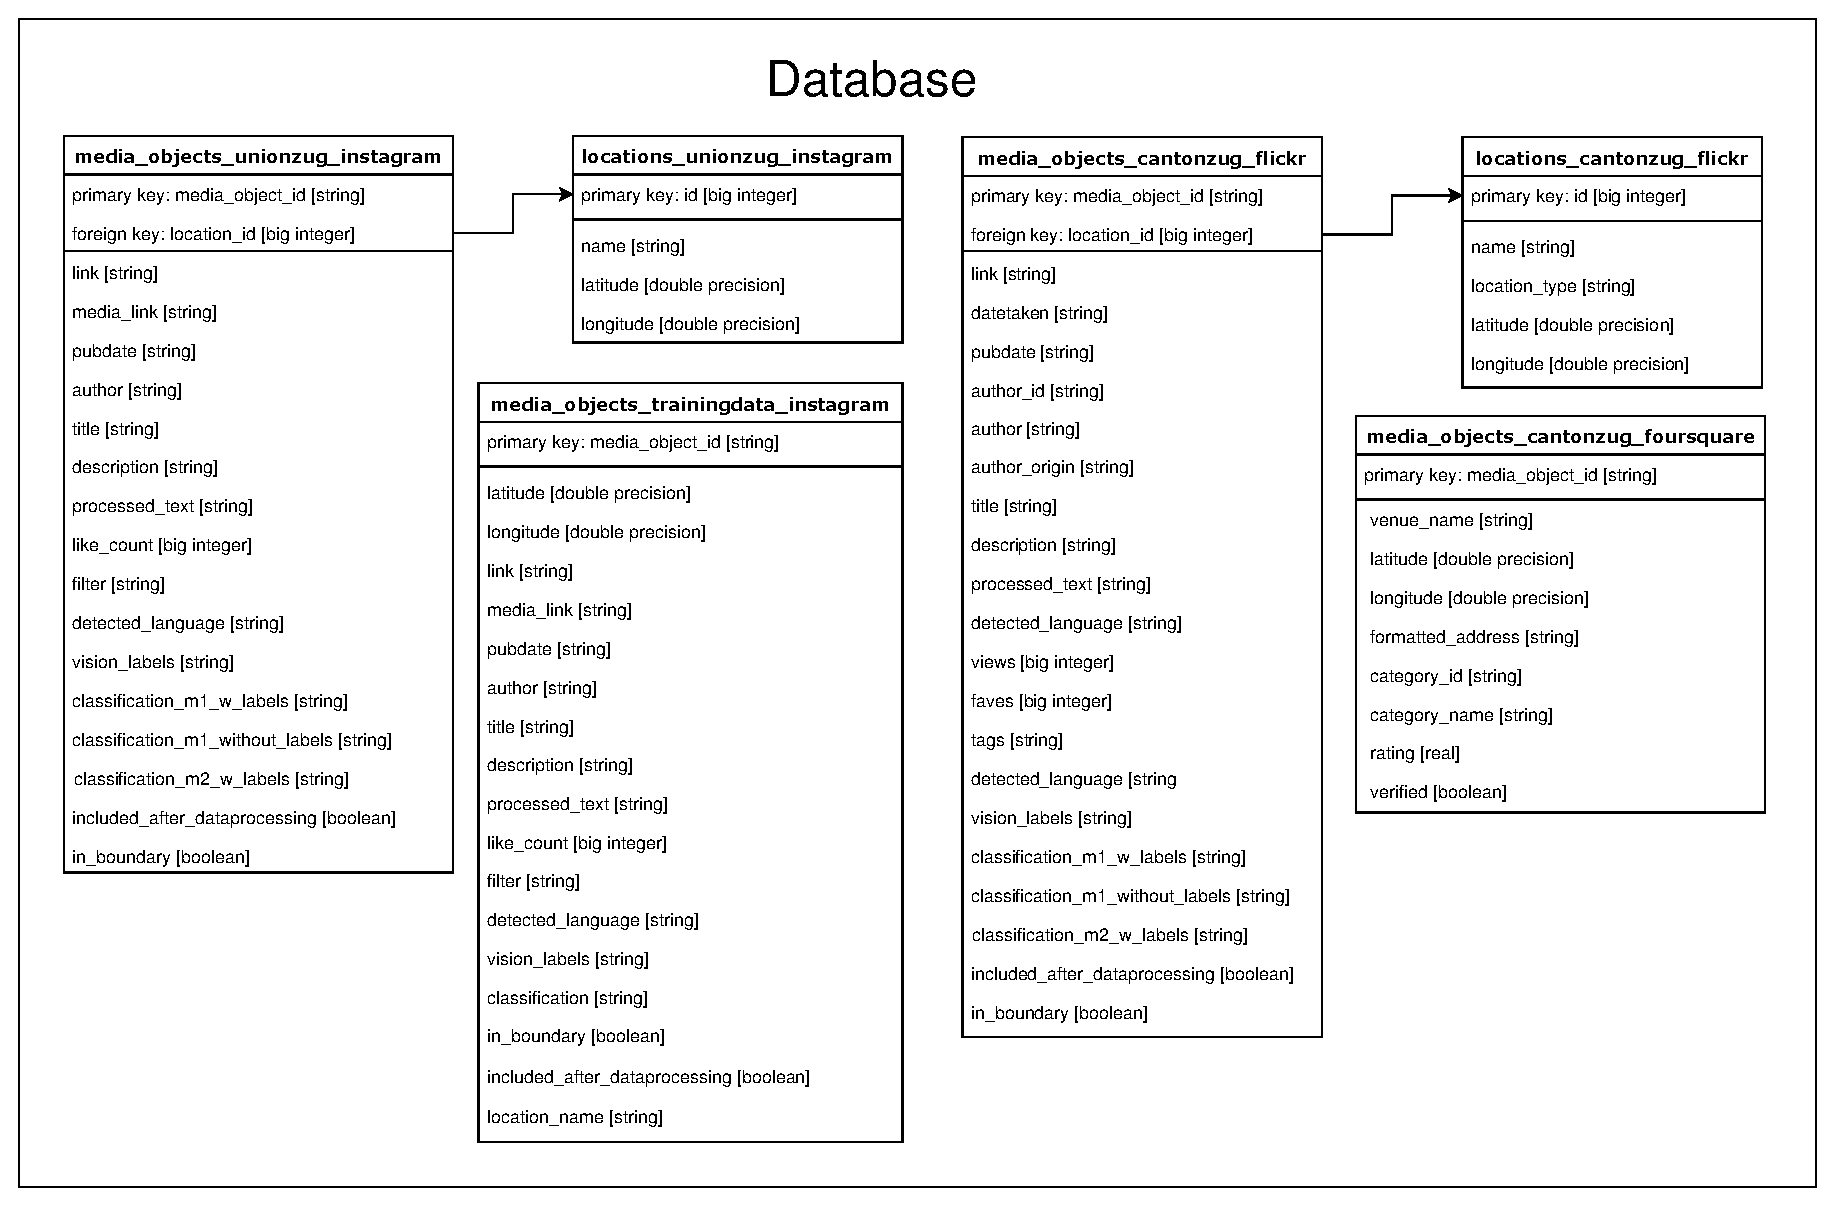
\includegraphics[width=\textwidth]{img/fusion_db_overview}
   \caption{Visualisation of the database, its associated tables and columns. \\ Created with https://www.draw.io/}
   \label{fig:database}
\end{figure}

\texttt{Remark:} The entire populated database in its final form can be found on the enclosed CD.

\section{Data-processing} \label{data_processing}
The following processes cover the entire workflow of data manipulation on the database in the order they were performed.
\subsection{Merging of Instagram files} \label{netlytic_files_merge}
In total, three different partly spatially overlapping Netlytic queries were run to acquire the needed Instagram data. All of them returned one CSV-file. These files were merged for simplicity reasons and media object duplicates were simultaneously removed in the process. This entire step was not needed for the Flickr-data since merging and duplicates were already handled during the data-mining process.

\subsection{Acquisition of additional location information} \label{add_location_data}
Auxiliary, more detailed location information regarding the spatial origin of the media objects in the database were acquired. The following two subsections will elaborate on this process for the different data sources Instagram and Flickr.

\subsubsection{Via the Instagram API} \label{geolocation_via_instagramapi}
The Instagram data that was provided by Netlytic was enhanced by using the \\ \texttt{GET/locations/location-id} endpoint of the official Instagram API. Newly acquired information encompassed the Instagram location-name.

\subsubsection{Via the Google Geocoding API} \label{geocoding_api}
Each coordinate of every Flickr media object was run through the Google Geocoding API. Detailed information regarding the media object's address and location type was returned. The location type attribute is evidence of the API's accuracy. Everything besides \small{\textit{ROOFTOP}} returns an address that is close but not exactly at the given coordinate and therefore represents a spatial approximation. The API has been called by modifying the following HTTPS-request:\\
\texttt{\footnotesize{https://maps.googleapis.com/maps/api/geocode/json?latlng=[latitude,longitude]\&key=[API\_KEY]}}

\subsection{Populating the database} \label{populate_db}
The merged Instagram CSV-files and the Flickr CSV-files which were extended by the additional location information described in the subsections above were used to populate the initial PostgreSQL database. This process was entirely performed with the script provided in Appendix \ref{python_code} and the needed \textit{psycopg 2} Python library that functions as linkage to the database.

\subsection{In boundary condition check} \label{in_boundary}
Additional unwanted data beyond the actual research area boundaries was included due to the circular (Netlytic; see figure \ref{research_area}) or rectangular (Flickr API) shape of the spatial query perimeters. As consequence each acquired media object was checked to be inside the actual perimeter boundary. This process was accomplished with an open source Geographical Information System (GIS) named QGIS. The point data of all media objects was clipped to the appropriate research area and exported to a new CSV-file. This CSV-file was read by the Python script which updated the \texttt{in\_boundary} column to \textit{True} for the provided media objects.

\subsection{Addressing sources of data-bias} \label{sources_data_bias}
This part of the data-processing is a filtering step as seen in step 1 of figure \ref{fig:ml_visualisation} to eliminate media objects which would distort the \textbf{general} perception of the research question at hand: Where are people performing NBRAs?

\subsubsection{Dominant authors} \label{bias_dominant_authors}
Authors (people who contribute to a given social media platform by uploading media objects) who are above a certain threshold regarding their total number of uploaded media objects in the research area during the data-acquisition period are marked in the database table column \texttt{included\_after\_dataprocessing} as \texttt{False} and are thereby excluded from further analysis. There is a need to address dominant authors because drawn conclusions will be otherwise based on a small number of users that contributed a large share to the entire data-set.\\
\newline
\textbf{How was this threshold defined?}\\
\newline
Two possibilities were considered:
\begin{enumerate}
  \item A static top percentage of authors will be excluded
  \item A variable dataset-specific amount of the most contributing authors will be excluded
\end{enumerate}

At first a static top 0.5\% threshold was implemented across all data-sets. Later in the development of the thesis possibility 2 was implemented. A 'posts per author' distribution graph (e.g. see figure \ref{img:dominant_users_flickr}) is simultaneously created as soon as data is read into the database. The number of desired top authors which should be included in the graph can be manually adjusted. This enabled a data specific dynamic adaption of the threshold according to a visual evaluation of the graph and the underlying dataset. 

\subsubsection{Bulk uploads} \label{bias_bulk_uploads}
In the context of this thesis bulk uploads describe a certain amount of simultaneously or during a short period of time uploaded media objects to the same social media platform by a single author. In an early stage of the project a static bulk upload threshold - similarly to the dominant author threshold - was chosen. Later, a dynamic solution which makes adaptive data handling possible was implemented. A graph which visualises the amount of effected media objects by different bulk upload thresholds (2-10) is displayed to the user (see figure \ref{img:bulk_uploads_flickr}). According to the graph a suitable threshold can be inputted and applied to the given dataset. The time period in which the exceeding of the threshold was considered a bulk upload was set to one hour. 
All as bulk upload marked media objects will be excluded from further analysis by setting the \texttt{included\_after\_dataprocessing} column to \textit{False} (if they were not already excluded in the 'dominant user' step).

\subsection{Text-processing} \label{text_processing}
Text processing is required to turn noisy user-generated character input (text) into normalised word-tokens which are comparable between media objects. These tokens are a prerequisite for the following machine learning (ML) text-classification approach. The text-processing encompasses the following steps in corresponding order which have been visualised under step 3 in figure \ref{fig:ml_visualisation}: Firstly, iterating over all media objects which lie inside the research area boundary and are included after the data-processing while acquiring the corresponding text-data from the database.

\subsubsection{Language detection} \label{language_detection}
The language detection serves the purpose of optimally adjusting the parameters for the later performed core text-processing step. By identifying the language, a matching word lists can be chosen to check the spelling, remove meaningless stop words as well as stem words to its roots (see \ref{core_text_processing}).\\
To accomplish a text string which consists of the media object's title is parsed to the function. Firstly, basic text-processing is necessary to ensure a reliable prediction which consists of splitting the text-string at white spaces. Next, any sort of URI (universal resource identifier), HTML, common geographic references (such as the city of Zug) and character/number combination-patterns are removed with the help of regular expression matching. Lastly, all characters are turned lowercase. The resulting word-tokens are only further considered if they have a minimum length of three characters. This minimum length was chosen according to conducted tests to avoid short character-artefacts that can occur during the described process.\\
In a following step each created word-token is run against five different word lists of the English, German, Swiss German, French and Italian language.
The English word list was acquired via the \textit{natural language toolkit} (NLTK) Python library. The mentioned list encompasses over 236'000 of the most common words of the English language.
The German, Swiss-German, French and Italian word lists\footnote{http://www.gwicks.net/dictionaries.htm, accessed: 29.03.2019} contain 166'100, 165'900, 208'913 and 88'351 of the most common words respectively.\\
\newline
\texttt{Remark:} All word lists were slightly modified to fit the text-processing algorithm that is applied to the text-data of the media objects (lowercase, replacement of vowel mutations).\\
\newline
The entity check of each word versus all five of the above mentioned word lists accounts for a major share of the total processing cost of the entire text-processing algorithm. The word list with the most contained words defines the language of the text string and ultimately of the entire media object. The determined language for each media object is saved in the 'detected\_language' column in the corresponding database entry.\\


\subsubsection{Core text-processing} \label{core_text_processing}
The core text processing encompasses the following alteration steps described in the following subsection and serves the purpose of creating universally similar structured and comparable word-tokens out of the noisy user generated text-data from each media object in the database. This entire process generates the feed-in-data which enables the training and testing of a sophisticated ML model to accurately predict the NBRA contained in the media objects.\\
The function \texttt{text\_processing\_core()} (see Appendix \ref{python_code}) is called with the matching word lists for spell checking, stop words exclusion and the correct stemmer object corresponding to the performed language detection. The provided text string consists of a concatenation of the media object's title and description unlike just the title for the shortened text processing algorithm applied in the language detection function.\\
Flickr tags were not neglected from this step even though they were also generated by an image detection algorithm similar to the Google Cloud Vision algorithm which was used in this thesis to acquire image content tags.

\paragraph*{Match and remove special text patterns} \label{text_patterns}
The first step of the text alteration included the regular expression matching (see definitions for reverence) of any URI (which includes \texttt{https://, http://, www.} beginnings as well as the domain ending), HTML related tags (e.g. \texttt{<a>\dots<$\backslash$a>}), Instagram mentions (e.g. \texttt{@madmax}) and character/number combination-patterns (e.g. \texttt{zugersee2018}). If detected they were replaced by a whitespace (\texttt{$\backslash$s}) character. This step was done prior to any other text-processing step due to the high risk of creating character artefacts which occur if those patterns remain in the text string.

\paragraph*{Removal of characters other than letters} \label{remove_eveything_but_letters}
As a next step all special characters such as Unicode characters of the category 'other symbols' including numbers were removed from the text string and also replaced by a whitespace (\texttt{$\backslash$s}) character. This assures that character objects like emojis, timestamps and dates that often occur in social media data are removed to reduce the noise in the list. Additionally, mutated vowels were replaced by a corresponding but simplified character sequence, e.g. '\"a' was replaced with 'ae'.

\paragraph*{Whitespace splitting} \label{whitespace_splitting}
Eventually the text string is split at the occurrence of one or more whitespaces. This creates for the first time individual word-tokens which will be further modified and filtered in the following steps.

\paragraph*{Spell-check} \label{spell_check}
Basic spell checking is done for the English, German and French language. The purpose again lies in the reduction of the vocabulary for the ML model. This is achieved by ensuring the same spelling and therefore the same token for a given word by reducing the variety created through spelling mistakes. Each given word-token is checked for being part of the same corresponding language word list (dictionary) already used for the determination of the media object language. If the token has been determined to be an exact entity of the given list it is returned without any alteration. If no match was found a suitable word correction is suggested by the algorithm. The entire process makes use of the Python library \textit{pyenchant} which handles the smart entity search as well as the word suggestion and word correction process. Spell checking was skipped for the Italian language due to a missing \textit{pyenchant} dictionary.

\paragraph*{Stemming} \label{word_stemming}
Stemming refers to the process of reducing a word to its linguistic root which yields many advantages for Information Retrieval (IR) in general and more particular for text-based ML models as demonstrated further down in section \ref{ml_text_data}. The following paper \textcite{Lovins1968} distinguishes between root and stem where the root is the stem minus any prefixes. This differentiation is not applied here. 
\textcite{Weissweiler2018} described the purpose of a stemmer as not being exclusive to finding the morphological correct root for a word but to reduce it to a form it shares with all words that are sufficiently semantically related. The exact nature of that form is irrelevant but it boils down to removing all prefixes and suffixes - leaving only the pure stem of the former word. Lemmatisation is another term that gets used in computational linguistics together with stemming. The difference being that lemmatisation considers the context of the entire sentence or document while algorithmically determining the lemma (stem) of a word. Stemming was used over lemmatisation due to the reduced processing cost which was a crucial criteria considering the data-volume.\\
While performing automated text analysis using ML algorithms stemming is important to enhance the performance of the model by merging tokens with similar meaning (e.g. different verb conjugates) to fewer resulting in an information gain per token. A model will not necessarily associate the same meaning and importance to different words even if they share the same stem. But rather will handle them as different features. Therefore, stemming is often applied to ML models that operate on heterogeneous user generated text.\\
In the field of stemming one can differentiate between dictionary-based and algorithmic stemmers. Former rely on finding the root of a word by hard scripting a dictionary and searching for a given word and return its associated root. These stemmers normally outperform the latter in terms of accuracy but they also have their drawbacks which is the reason why algorithmic stemmer still have purpose. Reasons being firstly computational cost - algorithmic stemmers require less time to run and can process around a million words in six seconds on a conventional 500MHz PC \parencite{Porter2001} which becomes increasingly important with growing data size. Despite the errors they make algorithmic stemmers still give good practical results. As \textcite{Krovetz1995} states in surprise of the algorithmic stemmer: "Why does it do so well?".\\ 
Secondly, dictionary-based stemmers require dictionary maintenance to keep up with an ever-changing language. It is not just that a dictionary created to assist stemming today will probably require major updating in a few years time but that a dictionary in use for this purpose today may already be several years out of date.\\
Due to the big dataset and its associated processing overhead as well as the unavailability of suitable dictionary-based stemmers four different algorithmic stemmers for the English, German, French and Italian language were used. Being able to apply the correct stemmer to a given text was the reason why a language detection was performed prior to the core text processing.\\
For the English, French and Italian language the Snowball Stemmer \parencite{Porter2001} with their respective language variation was used. Especially the English version has found wide acceptance in scientific applications such as \textcite{Krauthammer2011} or \textcite{Joulin2016} in the field of ML. This is among the reasons why this stemmer is part of the natural-language processing toolkit (NLTK) \parencite{Manning2014} of the used \textit{nltk} Python library.\\
For the German language however, stemmer variety and quality are comparably lower due to less attention. First tests were run with the German version of the above mentioned snowball stemmer which was later outperformed by a stemmer developed by the Ludwig-Maximilians University (LMU) Munich called CISTEM. The paper \textcite{Weissweiler2018} was published with the underlying algorithm source code which proves CISTEM's superior accuracy compared to similar stemmers (including the snowball stemmer) and a noticeable reduction in computation time.

\paragraph*{Conversion to lowercase and stripping of excess whitespace}
To maintain the uniformity of the word tokens every remaining character is turned lowercase and excess whitespace that could have occurred in the previous text-processing steps is removed once again.

\paragraph*{Minimum token length}
Setting a minimum word length adds an additional filter layer. Contextless word-tokens as well as character artefacts that were created throughout the text-processing steps are thereby neglected. The threshold was set to a minimum token-length of \textbf{three} for this thesis. In the English language only a few two letters words with contextual meaning exist besides stopwords such as 'or'. Words such as 'ad' (short for advertisement), 'ma' (short for mama/mother) or 'ou' (Hawaiian bird\footnote{https://birdsna.org/Species-Account/bna/species/ou/introduction, accessed: 08.04.2019}) are examples. Abbreviations or short-forms of other English words are predominant. The potential information gain for the model by including these words compared to the conjoined inflation of the feature space is considered to be low \parencite{Guido2016}.\\
\newline
\textbf{How was this threshold defined?}\\
\newline
This threshold was defined based upon personal empirical tests on the original data and on the book of \textcite{Guido2016}.

\paragraph*{Stop words}
Stop words describe a category of frequently used words that do not hold any strong contextual meaning which occur in every language. Examples for the English language are for instance the words: \textit{while}, \textit{before}, \textit{because}, \textit{theirs}.\\
English, German, French and Italian stop word lists - also provided by the \textit{nltk} Python library - which contained 179, 231, 155 and 279 (state: 23.11.2018) unique elements respectively were used for matching.\\
The reason for removing word tokens identified as stopwords is to prevent the inflation of the general word space while not proportionally enriching the overall contextual meaning of the entire text string. The more common words across different media objects are retained the more similar they seem to the ML model which hinders high prediction accuracies.

\paragraph*{Topographic related words}
Topographic names and descriptions from Switzerland were identified in the media object text and removed to ensures that the resulting model is not trained on specific geographic locations to avoid misleading associations when applying the model to a different area. Since the training data for this thesis originated from the Canton of Zurich and not from the actual research area this factor holds great importance. Accordingly, a list of towns and cities\footnote{http://data.geo.admin.ch/ch.swisstopo-vd.ortschaftenverzeichnis\_plz/PLZO\_CSV\_LV95.zip, accessed: 31.03.2019} and geographical names\footnote{https://shop.swisstopo.admin.ch/de/products/landscape/names3D, accessed: 31.03.2019} from the topographical survey of Switzerland are used for identification. 
The possibility to use this additional location information contained in these neglected topographic terms to further narrow down the location of the NBRAs was not considered. Further investigation in this regard is considered for future improvements to the method. Additionally, 20 language variations of the country name 'Switzerland'\footnote{https://www.101languages.net/countries/switzerland-in-other-languages/, accessed: 29.03.2019} where removed. \\
During the text-processing testing a crucial issue of location- and word-token names overlapping became apparent. Important action verbs among others of the German language such as 'laufen' (to walk) were being incorrectly removed based on the existing town 'Laufen' in Switzerland. To resolve this problem the list of topographic descriptions was run against the word dictionaries of the English, German, French and Italian language which were already used for the media object language detection. 1'032 matches on a total of 66'133 topographic list entities were the result. These words that hold both topographic and semantic meaning (see example above Laufen / laufen) were removed from the list of topographic deceptions and therefore remained in the text-corpora of the media objects.

\paragraph*{Feedback to the database}
The generated word-tokens and the identified language are saved in the database table columns \texttt{processed\_text} and \texttt{detected\_language} respectively where they are accessible for the ML training and testing phase.

\section{Image recognition} \label{image_recognition}
The extraction of structural elements from an image enables an additional information gain to further describe the overall context and content besides the user generated text. Since image recognition is a scientific field of its own a third-party service was used for this task. At the time of writing there were multiple suitable available solutions - two of which were the Amazon Rekognition Service and the Google Cloud Vision API. The latter was applied in this thesis based on the given pricing (see subsection \ref{vision_query_cost}) and initialisation conditions at that time. The Google Cloud Vision API allows users to draw upon a deep-learning algorithm that is constantly trained on Google's rich image pool to identify and classify structural elements in images.

\subsection{Process}
Every Flickr and Instagram media object stored in the database comes with a media link that allows direct access to the associated image. These links with the corresponding media object id's were iteratively queried and parsed to the Google Cloud Vision API for analysis. The basic processes is illustrated in figure \ref{fig:vision_illustration}\footnote{Source: (1) Mountain biker - https://allaboutlimassol.com/assets/images/primary-image/51024-0.downhill\_mountain\_biking.jpg, accessed: 30.03.2019 (2) Vision emblem - https://cloud.google.com/vision/?hl=de, accessed: 30.03.2019}. The output consists of text labels with their corresponding confidence score. These values are fed back into the \texttt{vision\_labels} database column of the row with the matching media object id the media link belonged to.

\begin{figure}[h!]
\centering
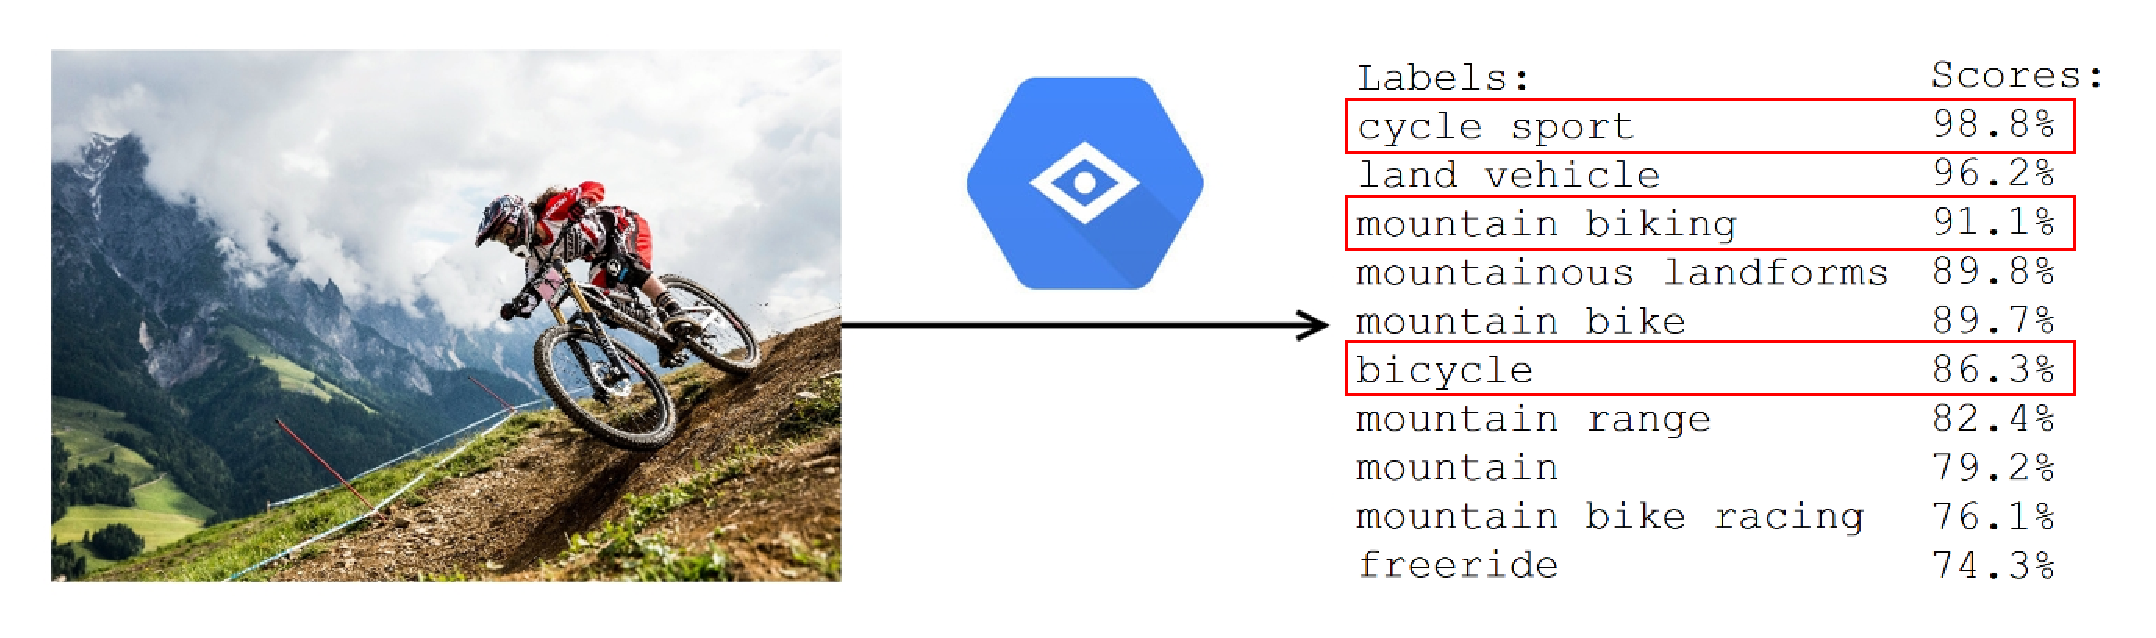
\includegraphics[width=0.75\textwidth]{img/vision_illustration}
\caption{This visualisation shall illustrate the image recognition process which is performed by the Google Cloud Vision API.}
\label{fig:vision_illustration}
\end{figure}

The placement of this entire step in relation to the other data- and text-processes is visualised in step 2 of figure \ref{fig:ml_visualisation}.

\subsection{Query costs} \label{vision_query_cost}
Google allows the creation of one Google Cloud trial account (needs a valid postpaid Credit Card for verification) per user which comes with 300 US Dollars' worth of credit. This credit can be used among others to rent virtual machines (VM's), access API's and other Google Cloud services.The Google Cloud Vision API can also be paid with that available credit and comes with the following rates: The first 1'000 requests per month are free of charge. Subsequent requests up to 5 million requests per month are charged at \$1.50 per 1'000 requests - this applies specifically to the API specific label detection feature. Therefore, the 300\$ worth of credit would allow the processing of around 201'000 images. These rates\footnote{https://cloud.google.com/vision/pricing, accessed: 29.03.2019} were in place during the time of writing (March 2019) and will mostly likely vary with time.

\clearpage

\section{Machine Learning for text classification} 

\subsection{Machine learning on non-numerical text data} \label{ml_text_data}

\begin{wrapfigure}{l}{0.3\textwidth} %0.3 and 0.28
  %\vspace{-0.5cm}
  %\begin{center}
    \centerline{\includegraphics[trim={0 0 0 0},clip,width=0.28\textwidth]{img/ML_text_data_visualization_cropped.pdf}}
%if trimming and clip is necessary: \includegraphics[trim={5cm 0 0 0},clip]{example-image-a}
  %\end{center}
  \caption{ML workflow}
  \label{fig:ml_visualisation}
\end{wrapfigure}

One approach to transform text-based data into machine readable information will be covered in this section. Steps 3, 4, 5 and 6 of figure \ref{fig:ml_visualisation} to the left can be used as reference and will illustrate the described processes.\\
There are multiple approaches available to prepare text-data for a ML model but outputting numbers at the end in one form or the other is uniform.\\
In this project the \textit{bag-of-words} representation has been applied \parencite{Joulin2016}. This algorithm learns the 'vocabulary' of a corpus of documents or media objects in this case. The entire corpus-vocabulary is compared to the word-tokens incorporated in each media object. Therefrom, a fingerprint-like sequence of numbers is created which represents the occurrence and absence of words-tokens in the corresponding media object. The entire process can be boiled down to three steps\footnote{https://scikit-learn.org/stable/modules/feature\_extraction.html\#text-feature-extraction, accessed: 29.03.2019} which explain more thoroughly what has been said above:

\paragraph*{Tokenization} The input consisting of the concatenated text strings and the image recognition labels of each media object is processed into word-tokens by a sequence of various functions as seen in section \ref{text_processing} \textit{Text-processing} and step 4 of figure \ref{fig:ml_visualisation}. N-grams (see \nameref{definitions}) upto \textit{n}=3 were considered during the tokenization procedure. This homogenisation enables a reduced model complexity by merging similar features and neglecting features with little semantic meaning. The generated string outputs (see \ref{fig:ml_visualisation} step 5) are fed into:

\paragraph*{Vocabulary building} By assessing the individual word-tokens of each media object the \textit{bag-of-words} constructor assembles a vocabulary of unique tokens found in the corpus. This vocabulary comes in the form of an alphabetic ordered array where each column represents a word token. These columns are from now on referred to as (model) features.

\paragraph*{Encoding} The previously build vocabulary array is iterated over and compared to the word tokens found in the final text-string of each media object for which a 'fingerprint'-array is instantiated. Missing words are recorded as nulls and appearances are recorded by their count. The final weight of each feature is calculated according to the \textbf{T}erm (feature) \textbf{F}requency inside the media object times the \textbf{I}nverse  \textbf{D}ocument  \textbf{F}requency (occurrence across all media objects) which is referred to as TF-IDF. This results in a number sequence linked to a given media object on which the model is later trained. The following equations illustrate how TF-IDF is calculated. T\textsubscript{d} stands for the number of times term 'T' occurs in document 'd', 'N' stands for the total number of documents and D\textsubscript{t} describes the amount of documents 'D' that contain term 't'.

\begin{align}
TF &= T\textsubscript{d}\\
IDF &= \log\frac{N}{D\textsubscript{t}}\\
TF-IDF &= T\textsubscript{d} * \log\frac{N}{D\textsubscript{t}}
\end{align}


TF-IDF was chosen over simple TF because it is assumed that terms that occur across multiple documents are frequently used words such as stopwords that do not hold significant information to classify and distinguish between the seven recreational activities. Trough this normalisation the identification of meaningful terms that appear in the majority of media objects of the same class such as 'walking' but rarely in miscellaneous media objects is possible. 

%\clearpage

\subsection{Recreation-types} \label{recreation_types}
The decision which NBRAs the model should capture was built upon and influenced by the 'Recreation types Guidebook' of the Institute of Technology Rapperswil \parencite{IFL2018}. The following seven distinct classes were chosen for the model to be trained on:
\begin{enumerate}
    \item walking
    \item hiking
    \item jogging
    \item biking
    \item dog walking
    \item horse riding
    \item picnic
\end{enumerate}
The observation of similar appearing classes is true and one can argue about its effectiveness and the degree of overlapping. How would people differentiate between e.g. walking, hiking and jogging? The ground truthing as well as the social media data revealed (see results \ref{results}) that some people perceive a journey through a forest as hiking while for others it is still considered going for a walk. Normally, NBRAs can be easily identified and distinguished by the needed equipment. Not so much in the case of the three mentioned NBRAs compared to the other classes like horse riding where you notably need a horse.\\
Nevertheless, the classes 1-3 account for the majority of recorded NBRA-occurrences. 77\% of the entire manually verified training data used to fit the model was classified as one of them. This clearly shows the importance of these NBRAs as well as their spatial distinction.
Additionally, a class 'None' is also implemented which describes a media object which is not related to nature recreation and therefore is not an entity of any of the above listed NBRAs.\\
\newline
The recreational activity 'swimming/bathing' that is listed in the recreation types guidebook by \textcite{IFL2018} was neglected for this thesis. The reasoning behind the exclusion is based on the Instagram data-acquisition period from the 30.09.2018 till the 11.12.2018. During this time little training data was available on outdoor swimming due to the low lake temperature. Additionally, the spatial occurrence of people swimming is less distributed and corresponds to certain well known locations. Considering these circumstances and the additional needed effort, the decision against the inclusion of 'swimming' as an independent class was made.

\subsection{Acquisition and preparation of the training- and test-dataset} \label{preparation_training_data}
Due to a limited amount of available Instagram and Flickr data of the research area and the entire Canton of Zug respectively it was certain that not enough training-data for each of the NBRA-types was available. Therefore, a larger additional Instagram dataset was drawn upon which was collected by the geocomputation team of the University of Zurich \parencite{Gruzd2016}. The dataset consists of ten locations in Switzerland which differed in topography, spoken language and demographic factors. The locations were the following: Aarau, Arosa, Ebmatingen, Locarno Nord, Neuch\^{a}tel, Ovronnaz, S-chanf, Scuol, Uetliberg and Zurich Dolder. For each location there existed around six to seven individual files that partly overlapped in the time they were acquired. The entire dataset covered a time-span of approximately three months for every of the mentioned locations from the beginning of October 2017 till the end of January 2018. A total of ten merge files - one for every location - were created to firstly eliminate any duplicate media objects and secondly to add the location name as an additional column to the data-rows for easier database filtering later on.\\

\begin{figure}[h]
   \centering
   \includegraphics[width=\textwidth]{img/TD_locations_cropped.pdf}
   \caption{The red circles indicate locations from which additional Instagram data as potential training data was available. The blue circles indicate the locations which were ultimately chose as training data sources. The green circle indicates the location of the research area.}
   \label{fig:TD_locations}
\end{figure}

After considering the different topographic attributes, the data-composition and quantity of all ten locations, Zurich Dolder and Uetliberg were chosen as sources for the training data due to their similarity to the research area and to the overall Canton of Zug. This accounted for a total of 206'454 and 74'742 unique media objects respectively during the pre-processing phase. After neglecting the top seven authors in the case of Zurich Dolder and the top ten for the Uetliberg dataset (see: \ref{bias_dominant_authors}) as well as applying a common bulk upload threshold of five uploads per day (see: \ref{bias_bulk_uploads}), this led to a dataset reduction to 191'584 and 68'522 post data-processing respectively. Attentive readers will notice that the resulting ML model is purely based on Instagram data even though Flickr data is predicted with it as well. This observation is correct and can be legitimatised with the assumption that user generated text does not differ to heavily between social media platforms. That this hypothesis hols true is shown in section \ref{precision_unseen_data}.\\
\newline
The next step encompassed the coarse identification of potential training data for the seven given NBRAs. This was done with tailored SQL queries (see Appendix \ref{sql_queries_for_trainingdata}) to the \texttt{processed\_text}-column of the \texttt{media\_objects\_trainingdata\_instagram} database-table containing case insensitive regular expressions (see definitions) in the form of:

\[processed\_text \sim * (\backslash s | \wedge)KEYWORD(\backslash s | \$)\]

The following break-down of the query explains the parameters and search criteria in more detail. The SQL syntax \texttt{$\sim$*} initiates a case-insensitive regular expression matching with the database \texttt{processed\_text}-column of each media object. A regular expression (short: regex) is a sequence of characters used to describe and match a specific string pattern. The regex \texttt{($\backslash$ s | $\wedge$)} defines that the string-pattern of interest must either start with a whitespace ($\backslash$ s) or must be located at the beginning of the string ($\wedge$). Next follows the placeholder for potential keywords that are likely to occur in a media object of interest of a certain class. The used keywords must be run through the same text-processing algorithm - the way every media object in the database did - to allow for successful matching. Lastly, ($\backslash$ s | \$) defines that the string-pattern must either end on a whitespace or must be located at the end of the string.\\ 
Media objects that were selected through this process were labelled according to the matching NBRA by changing the classification column in the corresponding row in the database. The order in which these NBRAs were queried impacted the amount of entities a given class would acquire after the entire set was classified. This is given by the fact that certain media objects fit the criteria of multiple queries or NBRAs. Therefore, an already classified media object could be reclassified by a later query. The order in which the queries were eventually executed corresponds to the order in the table below (see table \ref{tab:trainingsdata}). The idea behind this approach was to reduce reclassification of media objects that belonged to an already weakly represented NBRA in the training data such as 'horse riding' or 'dog walking'. Simultaneously, this would help even out the number of training data per classification which is sought-after for the ML training process. It has to be noted at this point that any media object that was not targeted by any of the class specific SQL queries was automatically assumed to be of the None-class which resembles media objects that are unrelated to any of the mentioned NBRAs.\\
These 1'890 coarse pre-determined classifications were manually verified in a following step and changed if needed. This led to a deduction to a total of 1'046 remaining training data objects (see \ref{tab:trainingsdata}). No media object with the pre-determined classification of 'None' was manually verified.\\
\newline
One issue that became apparent during the manual verification procedure was the problem of consistent class-definitions especially for classes that were closely related such as 'walking' and 'hiking'. As already touched upon before people tend to have different interpretations of what hiking and what walking is. Also hiking might sound more adventurous then walking which could explain an even more interchangeable usage in the field of social media. The following rules were established to differentiate between the three most similar classes: hiking, jogging and walking. A violation of these rules would lead to a reclassification during the manual verification process.

\begin{enumerate}
    \item Mentioned equipment: The presence of equipment related keywords in the media object text such as 'backpack' for the class 'hiking' are strong signals that favour a specific classification.
    \item Mentioned adjectives, adverbs: It is assumed that these NBRAs can be allocated on an axis that goes from relaxing to adventurous. Walking being on the far left, followed by jogging in the middle and hiking on the far-right side. If adjectives or adverbs are used, that allow the allocation of a media object on this axis, then the closest most fitting class is chosen.
    \item Basic human context interpretation: If a media object is incorrectly classified according to the (author of this thesis) human interpretation of the text then a reclassification is performed.
\end{enumerate}

The baseline being that the model is trained to capture the personal interpretation of the media object author of what he/she thinks the present NBRA is. Therefore, if no certain manual distinction between classes can be made then the used action verb decides the class, e.g.:\\
"We went for a walk on Uetliberg" $\to$ walking \\
"I went hiking on Uetliberg" $\to$ hiking\\
If multiple action verbs are present in the same media object that are specific to different recreation activities such as to the classes 'biking' and 'dog walking' in the phrase "Before we went biking we took the dog for a walk" then the media object classification was chosen according to the evident activity in the provided image. If the activity was not contained in the image then the most recent performed activity to the time the media object was uploaded was estimated and used for classification.

\begin{table}[ht]
\begin{center}
\caption{training data purification process}\vspace{1ex}
\label{tab:trainingsdata}
\begin{tabular}{llccc}\hline
NBRA & SQL query matches* & Classifications** & After manual verification \\ \hline
Walking & 549 & 485 & 333 \\
Hiking & 465 & 428 & 306 \\
Jogging & 377 & 358 & 208 \\
Picnic & 339 & 335 & 51 \\
Biking & 169 & 164 & 72 \\
Dog walking & 74 & 74 & 63 \\
Horse riding & 46 & 46 & 13 \\
None & - & 279'285 & 279'490 \\ \hline
\end{tabular}
\newline
*see Appendix **can get overwritten by other SQL queries
\end{center}
\end{table}

\subsection{Issue of expired Instagram media links} \label{expired_media_links}
Every media object acquired by the Instagram API or Netlytic contains a media link which points towards the embedded image, video itself. All these generated Instagram media links contain a timestamp component which functions as an expiration date upon which the links become invalid \parencite{Wayne2018}. At the time of writing the training dataset dates back more then one year and all the media links already turned invalid by now. \\ %It is important to note that this issue effects the reputability of this thesis since
The links to the full Instagram media object (see section \ref{Instagram_data}) on the other hand were still valid - given the author of the media object or Instagram themselves did not take it down in the meantime. The media link of interest could be acquired by crawling through the web-page and finding the HTML \texttt{<div>} container which encompassed the correct \texttt{<img>} element with the id = "FFVAD". The source (\texttt{src}) attribute of that image element provided a valid media link that could be passed directly to the Google Cloud Vision API for the image recognition.

\subsection{Machine learning model} \label{ml_model}
The following subsections encompass the entire pipeline of functions that were used to build \textbf{two} kinds of models. These models should provide insight on the effect of combining text and image content data in regards to model performance. Therefore, the first model was solely trained on the processed user generated text-data whereas the second model was trained additionally on the processed image content labels that were returned from the Google Cloud Vision API. Aside from that the models were setup, trained, tuned and implemented in exactly the same fashion.\\
Relevant scores for evaluating ML model performance are also introduced which are referenced again in the results. The entire code implementation of the subsequent steps can be found in Appendix \ref{python_code} and in digital form in the enclosed CD.

\subsubsection{Considered algorithms} \label{ml_algorithms}
The following algorithms were tested and evaluated for the creation of the two ML models. The results will be presented in section \ref{results_models}.

\paragraph*{Support Vector Machines (SVMs)}
A SVM can be used for classification and regression applications. Its aim is to divide media objects of different classes - represented as vectors - by creating a hyperplane while maximising the distance between the closest vectors of each class (see hyperplane H\textsubscript{2} in figure \ref{fig:SVM_visualisation}). This constraint improves the performance of the model on new data where vectors do not follow the exact spatial distribution of the training data.

\begin{wrapfigure}{l}{0.5\textwidth} %0.3 and 0.28
  %\vspace{-0.5cm}
  %\begin{center}
    \centerline{\includegraphics[trim={0 0 0 0},clip,width=0.28\textwidth]{img/Svm_separating_hyperplanes}}
%if trimming and clip is necessary: \includegraphics[trim={5cm 0 0 0},clip]{example-image-a}
  %\end{center}
  \caption{Visualisation of possible SVM fitted hyperplanes to separate two data-point clusters. H\textsubscript{3} does not manage to completely separate the clusters. H\textsubscript{1} does separate them entirely but violates the constraint to maximise the space between them, unlike H\textsubscript{2}. Source: https://en.wikipedia.org/wiki/ \\ Linear\_classifier, accessed: 29.03.2019}
  \label{fig:SVM_visualisation}
\vspace{-0.5cm}
\end{wrapfigure}

For the calculation of the mentioned hyperplane are only the marginal vectors of relevance because they define the border between the classes and therefore the location of the plane. Name giving is the fact that only a small portion of the entire vector set - the so called support vectors - is used for the training of the model. The result is an algorithm with comparably low processing costs.

\paragraph*{Decision Tree algorithm}
Like SVMs decision trees can be used if a continuous value (regression) or a concrete set of values (classification) is desired as model output. Decision trees are fundamentally consecutive IF / ELSE statements (nodes) which try to purify the data with increasing tree depth. The determination of the nodes operation and their position inside the tree is seen as the fitting or training of the model.\\
One specific variation of the generic decision tree which has been tested for this project is the so-called Random Forest. It creates a defined amount of individual decision trees which are trained on different random test- and train-splits of the training dataset. This process comes close to performing a cross-validation. At the end these trees are logically merged where deterministic features are kept and ones that carry little information are dropped. The result is a decision tree which more successfully captures the information contained in the training data while reducing the trend to overfitting.\\
Decision trees are prone to overfitting due to their infinite possible depth by adapting perfectly to any training dataset. This can be countered by limiting the maximal depth of the tree(s) (see listing \ref{coderandomForestparameters}) . This process is called pre-pruning.\\
\newline
 The book from \textcite{Guido2016} about ML stated that "Random Forests do not tend to perform well on very high dimensional, sparse data, such as text data". Nevertheless, the Random Forest algorithm was tested, evaluated and compared to the linearSVC visible in section \ref{results_models}. Due to the fact that the calculation process of the different decision trees can be multithreaded across all available CPU cores, the fitting process can be faster than the one of the linearSVC model (in this thesis roughly 15\% faster). 

\subsection{Model setup} \label{model_setup}
In addition to the previously mentioned data- and text-processing steps some extra functions were needed before the actual fitting algorithm could be applied. The models were setup with Python v.3.6.7 and the \textit{scikit-learn} library v.0.20.2. This library allowed pipelining\footnote{https://scikit-learn.org/stable/modules/compose.html, accessed: 29.03.2019} (see definitions) which consisted of the following functions:

\begin{enumerate}
    \item \textbf{TfidfVectorizer} Converts a collection of raw documents (media objects) into a matrix of TF-IDF features which stands for the frequency times the inverse document frequency of a given word-token (see step 5 and 6 of figure \ref{fig:ml_visualisation}). This function is equivalent to applying 'CountVectorizer' followed by 'TfidfTransformer'.\\
    \textit{Tuned hyper-parameters:}
    \begin{itemize}[label={}]
        \item \textbf{Min\_df} This parameter defines the minimal required document frequency of a word-token in the entire corpus to be included for further processing.
        \item \textbf{Ngram\_range} This parameter defines how word-tokens are interpreted by the model. Given a minimal and a maximal value the function is able to create new features by concatenating tokens that appear in succession. This enables the extraction of semantic meaning that would stay unseen if only individual token were considered \parencite{Surtikanti2013}. E.g (1,2) would consider all single tokens as well as the concatenation of two consecutive tokens. (2,3) would only consider token concatenations of length two up to a maximum of three.
    \end{itemize}
    
    \item \textbf{SelectKBest} This function allows for a further selection of the features generated by the vectorizer. Score functions such as ANOVA F-value and Chi-squared allow the selection of the most deterministic features in a set. Limiting the number of features can help to prevent model overfitting and increase a model's generalisation capabilities.\\
    \textit{Tuned hyper-parameters:}
    \begin{itemize}[label={}]
        \item \textbf{k} Defines the number of further considered features with the highest score.
    \end{itemize}
    
    \item \textbf{ML algorithm} LinearSVC and Random Forest classifiers (see section \ref{ml_algorithms}) were used to find the most well-rounded model.\\
    \textit{Tuned hyper-parameters:}
    \begin{itemize}[label={}]
        \item \textbf{LinearSVC \textit{C}} Adjusting this parameter gives the user control over the margin-size of the hyperplane. This effects how strong the model is fit to every single training point. Reducing this parameter allows for more generalisation and counteracts to overfitting. Increasing the 'C' parameter raise the model's training accuracy (see figure \ref{fig:over_underfitting}).
        
        \item \textbf{LinearSVC Penalty} This parameter introduces a regularisation penalty to prevent overfitting by minimising the components of the word-token vectors. There are two commonly used L\textsubscript{p}-norms:
        \begin{itemize}[label={}]
            \item \textbf{L1} Favours sparse parameter vectors which helps to identify important features.
            \item \textbf{L2} Forces parameter vectors to be close to zero.
            \item For more detailed information on these two regularisation terms with an in depth comparison please refer to \textcite{Mazilu2011}.
        \end{itemize}
        
        \item \textbf{Random Forest n\_estimators} Defines the amount of independent decision trees that are created. The higher the number the better are classification boundaries smoothed and the training data captured. The downside is the computational cost increase.
        
        \item \textbf{Random Forest max\_depth} Defines the number of levels the created decision trees are made of.
    \end{itemize}
    
    \item \textbf{GridSearchCV} This function allows the systematic testing of different hyperparameter settings to find the best performing configuration. This process is also known as model tuning. The weighted F1-score instead of the default accuracy score was used to evaluate performance of the individual models due to the multi-classification approach. Additionally, cross-validation is performed to ensure the result reliability (leave one out cross-validation has not been considered due to the great increase in processing time). The used hyperparameter testing grid for the Random Forest algorithm is visible in figure \ref{coderandomForestparameters} and the one for the linearSVC algorithm in figure \ref{codelinearsvcparameters}.
\end{enumerate}

%\begin{listing}
%\begin{minted}{python}
%randomforest_parameters = {
%                    'vect__min_df': [9, 10, 11, 12, 13, 14],
%                    'vect__ngram_range': [(1, 1), (1, 2), (2, 2), (1, 3)],
%                    'chi__k': [500, 600, 700, 'all'],
%                    'clf__max_depth': [5, 6, 7, 8, 9, 10, 11, 12, 13, None]
%                }
%\end{minted}
%\caption{Tuned hyperparameters of the Random Forest fitting algorithm}
%\label{coderandomForestparameters}
%\end{listing}

\begin{lstlisting}[language=Python, caption=Tuned hyperparameters of the Random Forest fitting algorithm, label=coderandomForestparameters]
randomforest_parameters = {
                    'vect__min_df': [9, 10, 11, 12, 13, 14],
                    'vect__ngram_range': [(1, 1), (1, 2), (2, 2), (1, 3)],
                    'chi__k': [500, 600, 700, 'all'],
                    'clf__max_depth': [5, 6, 7, 8, 9, 10, 11, 12, 13, None]
                }
\end{lstlisting}

\begin{lstlisting}[language=Python, caption=Tuned hyperparameters of the linearSVC fitting algorithm, label=codelinearsvcparameters]
linear_svc_parameters = {
                    'vect__min_df': [7, 8, 9, 10, 11, 12, 13],
                    'vect__ngram_range': [(1, 1), (1, 2), (2, 2), (1, 3)],
                    'chi__k': [500, 600, 700, 'all'],
                    'clf__C': [0.001, 0.1, 1, 10, 100]
                }
\end{lstlisting}

\texttt{Remark:} At the end the model was trained on the entire training dataset with the best parameter configuration.\\

\subsection{Evaluation scores} \label{ml_evaluation_scores}
There are different measurements to evaluate a ML model. All of them can be extracted from the confusion matrix created during the testing phase of the model. This matrix consists of rows that represent the actual classes and columns that represent the class predictions. The name confusion matrix stems from the purpose of noticing if the model is confusing classes.

\begin{wrapfigure}{LR}{0.5\textwidth} %0.3 and 0.28
  %\vspace{-0.5cm}
  %\begin{center}
 % \renewcommand{\thempfootnote}{\arabic{mpfootnote}}
    \centerline{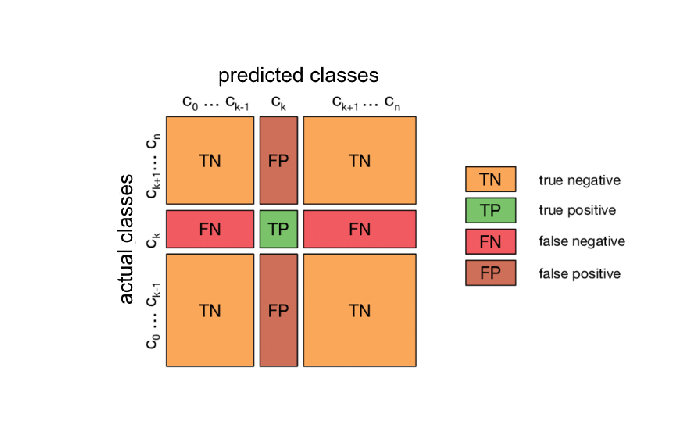
\includegraphics[trim={0 0 0 0},clip,width=0.49\textwidth]{img/Confusion_matrix_edited}}
%if trimming and clip is necessary: \includegraphics[trim={5cm 0 0 0},clip]{example-image-a}
  %\end{center}
  \caption{Confusion matrix with \textit{n} classes. When considering the class k (0 $\le$ k $\le$ n), the four different classification results can be obtained: true positive (green), true negative (orange), false positive (brown, Type I error), and false negative (red, Type II error). Source: https://www.researchgate.net/figure/Confusion-matrix-for-multi-class-classification-The-confusion-matrix-of-a\_fig7\_314116591, author: Frank Kr\"uger, accessed: 29.03.2019}
  \label{fig:confusion_matrix_illustration}
\end{wrapfigure}

Measurements that were calculated (Abbreviations explained in the legend of figure \ref{fig:confusion_matrix_illustration}):

\begin{gather*}
accuracy = \frac{(TP+TN)}{(TP+TN+FP+FN)}\\
precision = \frac{TP}{(TP+FP)}\\
recall = \frac{TP}{(TP+FN)}\\
F1 = 2*\frac{(precision*recall)}{(precision+recall)}
\end{gather*}

\textit{F1-Score: Summarising Precision and Recall in one measurement.}

\clearpage

\section{Ground truthing} \label{groud_truthing}
Interviews and passive observations were performed to gain insight on how well the social media data approximates to actual visitation rates and spatial NBRA dispersion. This ground truth information shall help to answer the question on how good of a proxy the considered social media platforms and their data in the study area are.

\subsection{Locations for ground truth data acquisition} \label{locations_ground_truthing_data}

\begin{wrapfigure}{LR}{0.4\textwidth} %0.3 and 0.28
  %\vspace{-0.5cm}
  %\begin{center}
    \centerline{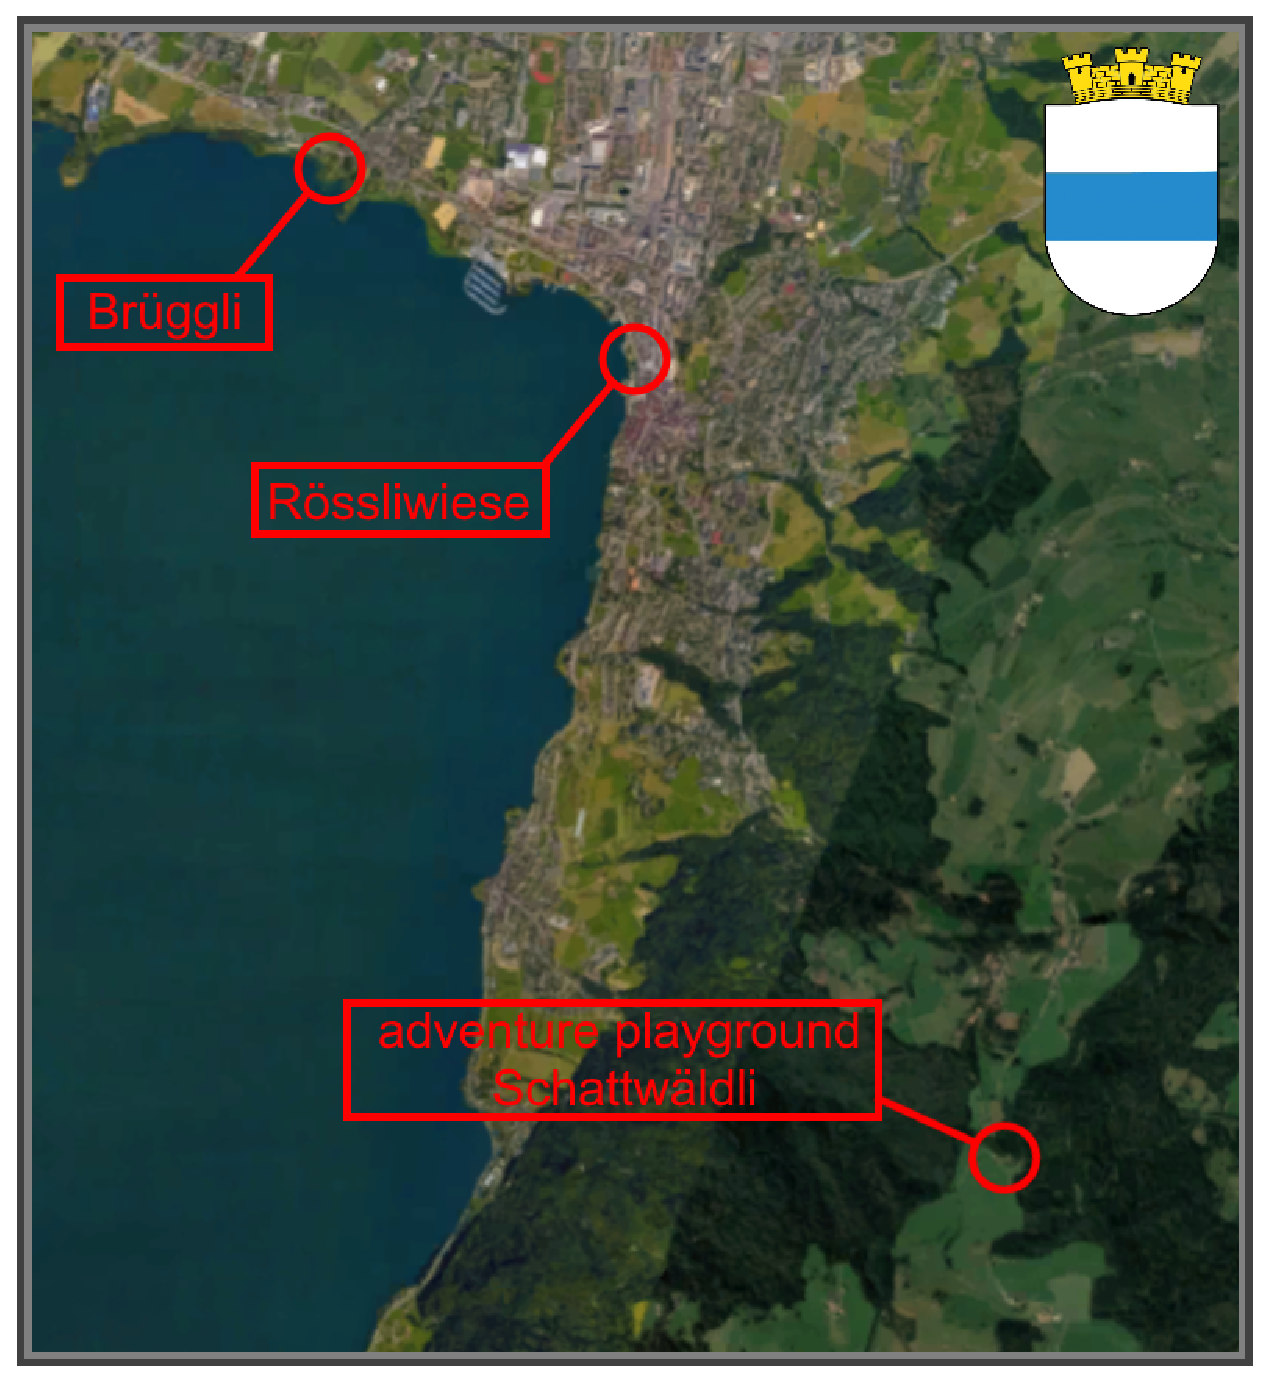
\includegraphics[trim={0 0 0 0},clip,width=0.39\textwidth]{img/interviews_locations}}
%if trimming and clip is necessary: \includegraphics[trim={5cm 0 0 0},clip]{example-image-a}
  %\end{center}
  \caption{Map visualising the locations where ground truthing in the form of interviews and passive NBRA observations were performed. Source: \copyright Google, map-data 2019}
  \label{fig:locations_ground_truthing}
%\vspace{-0.5cm}
\end{wrapfigure}

Three locations (see figure \ref{fig:locations_ground_truthing}) with different degrees of urbanisation were chosen which resemble hotspots for NBRAs covered in this thesis. The location to the far left is called 'Br\"uggli' - right next to a camping ground - which resembles a hotspot for jogging, biking, (dog-) walking and in summer also for picnicking and swimming. It lies inside the perimeter of the concept 'Lorzenebene' (plain of the river Lorze) and is close to the 'Delta' wildlife sanctuary which allows for various activities along the lake for relaxation.\\
The second location includes the 'R\"ossliwiese' which is a meadow located close to the city centre at the lake side. There people like to go for short walks (with their dog), eat lunch, relax (after shopping). Its high attractiveness is mostly given by the closeness to the residential area.\\
The last and most nature-near location was the adventure playground 'Schattenw\"aldli' on the Zugerberg. It appeals to various groups of people due to its wide spectrum of activities the environment allows. Young families with kids are the most dominant visitor group due to the playground and the possibility to have a picnic. But also people hiking, walking (their dog) and mountain-bikers can be frequently encountered there.

\subsection{Passive observation setup} \label{passive_observation_setup}
The passive observation encompassed the recording of NBRAs performed by people that passed through the location during the same time the interviews were held. More specific the group size, the approximate average group age, the NBRA and the time were captured. The term 'passive' implies that no direct interaction with the recorded people occurred. Therefore, the data is entirely based on perception.
Since the thesis's author held all the interviews, the passive observation was performed by an unaffiliated assistant (see \nameref{acknowledgements}).\\
The durations of these passive observations were the following:
\begin{itemize}
    \item \textbf{Br\"uggli} 1h 30min
    \item \textbf{R\"ossliwiese} 1h 15min
    \item \textbf{Schattenw\"aldli} 1h 45min
\end{itemize}
The time spent in one location depends on the time needed to hold the required interviews owing to the observable differences. Also, the relation between the observed frequencies of NBRAs were of greater interest than the actual recorded numbers.
The passive observation template used in this thesis can be found under Appendix \ref{passive_obs_templates}.

\subsection{Interview setup} \label{interview_setup}
A total of \textbf{52} interviews were performed in the afternoon during slightly cloudy but sunny conditions on the 24\textsuperscript{th} in 'Br\"uggli' (18 interviews) and 'R\"ossliwiese' (17 interviews) as well as on the 25\textsuperscript{th} of November 2018 in 'Schattenw\"aldli' (17 interviews). It was tried - to the best abilities of the author - to interview homogeneously across different age groups and NBRAs.\\
Every interview started out with a small introduction to the author's persona and the motivation behind the interviews. Additionally, the interviewees were informed that all the gathered information will be kept anonymous and used only within the scope of this thesis. The purpose of these interviews was to gain information on three topics.\\
\newline
The first one being \textbf{location} related:
\begin{itemize}[label={}]
    \item \textbf{Reason} Why was the current location in particular sought out? What was the motivation that resulted in visiting this location over another?
    \item \textbf{Activity} Which recreational activity is currently practised by the person in this location?
    \item \textbf{Frequency} How often does the person visit the location? (In the case of 'Schattenw\"aldli', it was also asked what the destination of the trip was.)
\end{itemize}

The second one was related to \textbf{social media}:
\begin{itemize}[label={}]
    \item \textbf{Member} Do they own an account on any social media platform and if yes on which?
    \item \textbf{Habits} How do they interact with social media? Do they share own content (if yes in what frequency?), or do they rather look at contributions of others?
    \item \textbf{Intent} Do they consider sharing their current visit to the given location on social media and if yes on which platform?
\end{itemize}
The final topic at the end of the interview was dedicated to some person specific details. This included their age, gender, place of residence as well as the travel time to the location and their choice of transportation.\\
The interview template used in this thesis can be found under Appendix \ref{interview_templates}.

\subsection{Data-comparison procedure}
The ground truth data was acquired to compare recreational activity occurrences from empirical \textit{in-situ} data and from social media data. This comparison provides insight on how well these two data-sources complement each other or where they show agreement. Additionally, the social media behaviour of the interviewees sheds light on the demographics of users that contribute to the social media platforms that were used in this thesis. This information allows statements about the representative of the produced models compared to real world circumstances.

\paragraph*{Recreational activities \& infrastructure}
The two data-sources were quantitatively compared according to the inferred ranking of recreational activity occurrences at the three locations where ground truth was acquired. The Spearman's Rank-Order Correlation was used for the statistical analysis of the rankings. Total observation numbers did not yield a good measure of comparison since the data-acquisition periods for both data-sources were incomparable. 

\paragraph*{Social media usage}
The 52 interviewees are considered a representational sub-sample of the range of users found in the research area. The inferred demographics from the interviews such as age and gender will be compared to social media platform specific demographic statistics\footnote{https://napoleoncat.com/stats/, accessed: 09.04.2019} to investigate their agreement and differences. Knowing how well the social media data coincides with the ground truth allows statements about Instagram's and FLickr's proxy potential to predict NBRAs. Knowing what share of the population is under- or over-represented by the used social media platforms enables future projects to merge empirical \textit{in-situ} data with UGC to cover a broader spectrum of the population.\\
Additionally, the social media behaviour of the interviewees yielded a ranking of most frequently used social media platforms. This information allowed to evaluate the appropriateness of using Instagram and Flickr data above other UGC-sources in this thesis.

\paragraph*{Visitation motivation}
The given reasoning why certain locations were preferably visited above others was considered a valuable byproduct of the interviews and shall provide the spatial planning agency of the Canton of Zug and other researchers with information about place preference. Since visitation motivation was not directly extracted from the social media data a comparison between the two data-sources was not conducted.

















%\input{chapters/howto}
\cleardoublepage
\chapter{Results} \label{results}
This chapter will encompass the result of the two ML models for NBRA prediction in Instagram and Flickr media objects as well as the evaluation of the in-situ interviews and the passive observation statistic of NBRAs.
\section{Data-processing} \label{results_dataprocessing}
The following table \ref{tab:data_reduction_values}will provide data-reduction values for each data-source and dataset used. These reductions were the result of the different data-processing steps described in \ref{data_processing} which will be shortly listed again below:
\begin{itemize}
  \item in boundary check
  \item dominant authors exclusion
  \item bulk uploads
\end{itemize}

\begin{table}[h!]
\begin{center}
\caption{Data-reduction according to the different data-sources as a result of data-processing steps}\vspace{1ex}
\label{tab:data_reduction_values}
\begin{tabular}{ccccc}\hline
dataset & excluded top authors & bulk threshold & input & output & data-reduction\\ \hline
Instagram Zug & 6 & 6 & 28'246 & 11'777 & 58.3\% \\
Instagram Zurich Uetliberg & 10 & 5 & 74'742 & 68'522 & 8.3\% \\
Instagram Zurich Dolder & 7 & 5 &  206'454 &  191'584 & 7.2\% \\
Flickr Zug & 12 & 7 &  14'236 &  3'790 & 73.4\% \\ 
Foursquare Zug & - & - & 405 & 405 & 0.0\% \\ \hline
\end{tabular}
\end{center}
\end{table}

The noticeably high data-reduction of the Flickr dataset was mostly due to high user upload activity. As seen in figure \ref{img:dominant_users_flickr} a small portion of Flickr-users (authors) uploading up to  1'190 posts since the SMP Flickr was launched in 2005 account for a big share of the entire dataset. As a result to reduce this bias, roughly 5'700 media objects were removed alone in the 'dominant user' data-processing step.\\
Similar graphs to figure \ref{img:dominant_users_flickr} were created for all the datasets according to which the thesis author decided the thresholds in \ref{tab:data_reduction_values} manually. 

\begin{figure}[h!]
   \centering
   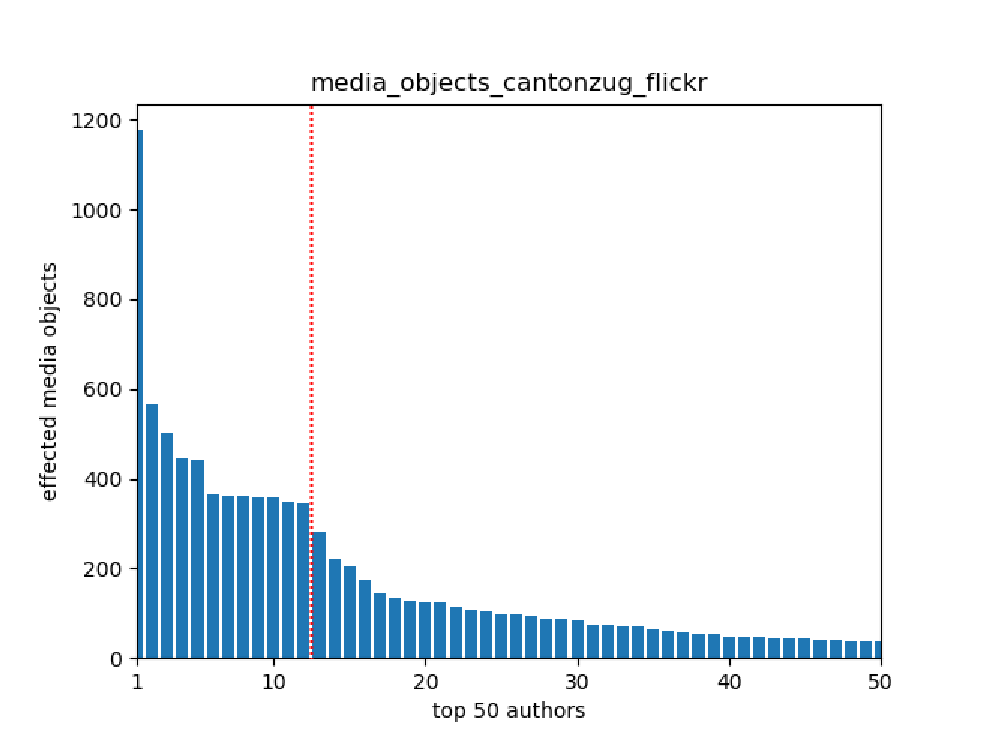
\includegraphics[width=0.75\textwidth]{img/cantonzug_flickr_top50_w_line}
   \caption{The top 12 Flickr authors which account for roughly 5'700 media objects (left to the red line) were excluded from further data-analysis}
   \label{img:dominant_users_flickr}
\end{figure}

\section{Models} \label{results_models}
The following subsections will cover the  performance results of each of the two created models (see chapter \ref{ml_model} that were solely trained on the Instagram Zurich Dolder and Instagram Zurich Uetliberg datasets included in the database table:\\ \texttt{media\_objects\_trainingdata\_instagram} (see figure \ref{database_setup}). For each model the random forest classifier and the linearSVC fitting algorithm was independently tested. The hyperparameters were tuned to yield the best possible average F1-score over all classes excluding the None-class. Simultaneously, the effect of including different amounts of the None-class training's data media objects during model fitting were also investigated. These values ranged from 500 to 6'500 with steps of 500.\\
These models were then used to predict the NBRAs contained in the media objects of the Instagram database table: \texttt{media\_objects\_unionzug\_instagram} and the \\Flickr database table: \texttt{media\_objects\_cantonzug\_flickr} from the Canton Zug.\\
Each model performed two separate predictions on each of the above mentioned datasets which differed in the final text-string composition that was parsed for prediction. One time the final text-string was constructed by concatenating the processed text-data and the image labels of a given media object. The second time the final text-string only contained the processed text-data.

\texttt{Remark:} The entire data presented in the following subchapters is available on the enclosed CD to this thesis. This includes the actual M1 and M2 dump files, tuning and cross-validation logs as well as the most important performance graphs (see chapter \ref{CD_content}).

\subsection{Model 1: untrained on image labels}
The first model (M1) that was trained exclusively on the processed user generated text-data (see chapter \ref{text_processing}). Therefore, it did not include any information about the image and its content. This leads to the model vocabulary potentially missing the associated image labels that the image recognition would yield.

\subsubsection{M1 - Random forest}
The model tuning with the parameter grid visible in figure \ref{code:randomForest_parameters} resulted in the following best hyper-parameter performing constellation:\\

\begin{table}[h!]
\begin{center}
\caption{Best hyperparameter setting for the random forest algorithm. The parameter descriptions can be found in Chapter \ref{model_setup}}\vspace{1ex}
\label{tab:m1_randomForest_bestParams}
\begin{tabular}{ccccc}\hline
k & max\_depth & min\_df & ngram\_range & none\_objects \\ \hline
all & None (no restriction) & 11 & (1, 1) & 3'500 \\ \hline
\end{tabular}
\end{center}
\end{table}

This hyper-parameter setting visible in the table \ref{tab:m1_randomForest_bestParams} allowed for the best model performance with a resulting number of \textbf{727 features}. All scores listed in table \ref{tab:m1_randomForest_bestscores} were rounded to three decimal places and were calculated with the scikit-learn 'weighted' parameter. The 'F1-score'-column refers to the weighted average across all classes whereas the 'F1-score without none class' refers to the weighted average across all classes except the none class.

\begin{table}[h!]
\begin{center}
\caption{M1 random forest performance scores during testing (except accuracy train)}\vspace{1ex}
\label{tab:m1_randomForest_bestscores}
\begin{tabular}{cccccc}\hline
Accuracy train & Accuracy test & Precision & Recall & F1 & F1 (without none class)\\ \hline
0.999 & 0.941 & 0.941 & 0.941 & 0.936 & 0.757 \\ \hline
\end{tabular}
\end{center}
\end{table}

\subsubsection{M1 - LinearSVC}
The model tuning with the parameter grid visible in figure \ref{code:linear_svc_parameters} resulted in the following best performing hyperparameter constellation:

\begin{table}[h!]
\begin{center}
\caption{Best hyperparameter setting for the linearSVC algorithm. The parameter descriptions can be found in chapter \ref{model_setup}}\vspace{1ex}
\label{tab:m1_linearSVC_bestParams}
\begin{tabular}{llccc}\hline
k & C & min\_df & ngram\_range & none\_objects \\ \hline
all & 1 & 12 & (1, 1) & 3'000 \\ \hline
\end{tabular}
\end{center}
\end{table}

This hyper-parameter setting visible in the table \ref{tab:m1_linearSVC_bestParams} allowed for the best model performance with a resulting number of \textbf{626 features}. All scores listed in table \ref{tab:m1_linearSVC_bestscores} were rounded to three decimal places. The 'F1-score'-column refers to the weighted average1 across all classes whereas the 'F1-score without none class' refers to the weighted average1 across all classes except the none class.

\begin{table}[h!]
\begin{center}
\caption{M1 linearSVC performance scores during testing (except accuracy train)}\vspace{1ex}
\label{tab:m1_linearSVC_bestscores}
\begin{tabular}{cccccc}\hline
Accuracy train & Accuracy test & Precision & Recall & F1 & F1 (without none class)\\ \hline
0.983 & 0.937 & 0.937 & 0.937 & 0.937 & 0.870 \\ \hline
\end{tabular}
\end{center}
\end{table}

\subsection{Model 2: trained on image labels and text-data}
The second model (M2) was trained on the Google Cloud Vision API image labels and the processed user generated text-data (see chapter \ref{text_processing}).

\subsubsection{M2 - Random forest}
The model tuning with the parameter grid visible in figure \ref{code:randomForest_parameters} resulted in the following best hyper-parameter performing constellation:\\

\begin{table}[h!]
\begin{center}
\caption{Best hyperparameter setting for the random forest algorithm. The parameter descriptions can be found in Chapter \ref{model_setup}}\vspace{1ex}
\label{tab:m2_randomForest_bestParams}
\begin{tabular}{llccc}\hline
k & max\_depth & min\_df & ngram\_range & none\_objects \\ \hline
all & None (no restriction) & 14 & (1, 1) & 400 \\ \hline
\end{tabular}
\end{center}
\end{table}

This hyper-parameter setting visible in the table \ref{tab:m2_randomForest_bestParams} allowed for the best model performance with a resulting number of \textbf{324 features}. All scores listed in table \ref{tab:m2_randomForest_bestscores} were rounded to three decimal places and were calculated with the scikit-learn 'weighted' parameter. The 'F1-score'-column refers to the weighted average across all classes whereas the 'F1-score without none class' refers to the weighted average across all classes except the none class.

\begin{table}[h!]
\begin{center}
\caption{M2 random forest performance scores during testing (except accuracy train)}\vspace{1ex}
\label{tab:m2_randomForest_bestscores}
\begin{tabular}{cccccc}\hline
Accuracy train & Accuracy test & Precision & Recall & F1 & F1 (without none class)\\ \hline
0.998 & 0.892 & 0.903 & 0.901 & 0.892 & 0.745\\ \hline
\end{tabular}
\end{center}
\end{table}

\subsubsection{M2 - LinearSVC}
The model tuning with the parameter grid visible in figure \ref{code:linear_svc_parameters} resulted in the following best performing hyperparameter constellation:

\begin{table}[h!]
\begin{center}
\caption{Best hyperparameter setting for the linearSVC algorithm. The parameter descriptions can be found in chapter \ref{model_setup}}\vspace{1ex}
\label{tab:m2_linearSVC_bestParams}
\begin{tabular}{llccc}\hline
k & C & min\_df & ngram\_range & none\_objects \\ \hline
all & 1 & 7 & (1, 1) & 700 \\ \hline
\end{tabular}
\end{center}
\end{table}

This hyper-parameter setting visible in the table \ref{tab:m2_linearSVC_bestParams} allowed for the best model performance with a resulting number of \textbf{775 features}. All scores listed in table \ref{tab:m2_linearSVC_bestscores} were rounded to three decimal places. The 'F1-score'-column refers to the weighted average1 across all classes whereas the 'F1-score without none class' refers to the weighted average1 across all classes except the none class.

\begin{table}[h!]
\begin{center}
\caption{M2 linearSVC performance scores during testing (except accuracy train)}\vspace{1ex}
\label{tab:m2_linearSVC_bestscores}
\begin{tabular}{cccccc}\hline
Accuracy train & Accuracy test & Precision & Recall & F1 & F1 (without none class)\\ \hline
0.993 & 0.882 & 0.883 & 0.886 & 0.882 & 0.835 \\ \hline
\end{tabular}
\end{center}
\end{table}

\subsubsection{Best features}
The following figure \ref{fig:M2_top40_features_biking} visualises the 40 most predictive features of the class 'Biking'. Similar figures for the remaining classifications 'Walking', 'Hiking', 'Jogging', 'Dog walking', 'Horse riding', 'Picnic' and 'None' can be found in appendix \ref{M2_top_features}. 
\begin{figure}[h!]
   \centering
   \includegraphics[width=\textwidth]{img/m2_top_40_features_Biking_cropped.pdf}
   \caption{Most predictive 40 M2-features of the class 'Biking'. Blue features are word-tokens which supports the presence of the corresponding classification. Red features support the opposite. The graphic was created with the \textit{mglearn} Python library provided by \parencite{Guido2016}}
   \label{fig:M2_top40_features_biking}
\end{figure}

\subsection{Model comparison}
In the following subsections, the above presented models will be thoroughly compared in terms of classification specific aspects, hyperparameter behaviour and performance on unseen data (data the models were not trained on). 

\subsubsection{Hyperparameter interaction}
The effect of different ngram\_range settings in combination with varying C values is illustrated in figure \ref{fig:heatmaps} for M1 and M2 respectively. The red circles indicates the highest F1-score present which corresponds to the best hyperparameter setting of the respective model (see table \ref{tab:m2_linearSVC_bestParams}). It becomes apparent, that the (2, 2) ngram\_range as well as the C value 0.01 underperform across the board. The F1-scores in the heatmaps are not completely identical to the values found in the corresponding model performance tables \ref{tab:m1_linearSVC_bestscores} and \ref{tab:m2_linearSVC_bestscores}. This variation is due to randomisation effects of the none-object selection from the database as well as from the model train and test splits (this is partly taken care of by cross-validation).\\

\begin{figure}[h!]
 \begin{subfigure}{0.5\textwidth}
   \centering
   \includegraphics[width=0.9\linewidth]{img/m1_F1_ngram_C_heatmap_w_Circle.pdf}
   \caption{M1 linearSVC}
   \label{fig:m1_heatmap}
\end{subfigure}
\begin{subfigure}{0.5\textwidth}
   \centering
   \includegraphics[width=0.9\linewidth]{img/m2_ngram_C_heatmap_new_w_circle.pdf}
   \caption{M2 linearSVC}
   \label{fig:m2_heatmap}
 \end{subfigure}
\caption{These heatmaps shows cross-validated F1-scores dependent on different combinations of the hyper-parameters ngram\_range and C for the model M1 (a) and M2 (b). These graphs were created with the Python library \textit{mglearn} from \parencite{Guido2016}}
\label{fig:heatmaps}
\end{figure}

\texttt{Remark:} If different hyperparameter settings produce the same model performance (F1-score) than the setting which produces fewer features is prioritised due to better generalisation capabilities. Regarding figure \ref{fig:m1_heatmap} for instance, the n\_gram setting of either (1, 1), (1, 2) or (1, 3) in combination with C = 1 all produce a F1-score of 0.932. (1, 1) has been chosen as best hyperparameter configuration due to the lowest feature count.

\subsubsection{Classification specific F1-scores}

\begin{figure}[h!]
   \centering
   \includegraphics[width=\textwidth]{img/m1_m2_class_f1_scores_bigger_font.pdf}
   \caption{Comparison of the classification specific F1-scores of the linearSVC and random forest fitting algorithm of M1 and M2}
   \label{fig:m1_m2_class_f1_scores}
\end{figure}

\subsubsection{Final model scores}
In the end the model M1 and M2 were trained on the entire training's dataset which resulted in the following final performance scores visible in table \ref{tab:m1_m2_linearSVC_final_scores}. This step is important to generate a final model that is eventually trained on as much training's data as possible. Keeping a portion of the training's dataset aside for model validation is no longer necessary because the most well performing hyperparameter configuration was already determined before.\\
\newline
It can be noted at this point that the best M1 and M2 performance yielded similar feature counts during testing (626 and 775 respectively) and after training it on the entire dataset (845 and 958 respectively).  
\begin{table}[h]
\begin{center}
\caption{M2 linearSVC performance scores during testing (except accuracy train)}\vspace{1ex}
\label{tab:m1_m2_linearSVC_final_scores}
\begin{tabular}{cccccc}\hline
Model & Accuracy & Precision & Recall & F1 & F1 (without none class) & Features\\ \hline
M1 & 0.984 & 0.984 & 0.984 & 0.984 & 0.967 & 845\\
M2 & 0.991 & 0.991 & 0.991 & 0.991 & 0.993 & 958\\ \hline
\end{tabular}
\end{center}
\end{table}

\subsubsection{Precision on unseen data}
This section will present the results of the model performance on new data. All Instagram and Flickr media objects of the Canton of Zug on which these results are based were excluded from the M1 and M2 model training.\\
Two separate predictions per model were performed on the media objects contained in the following two database-tables (database overview: \ref{database_setup}):
\texttt{media\_objects\_unionzug\_instagram} \\ \texttt{media\_objects\_cantonzug\_flickr}

One time the final text-string provided for the prediction was constructed by concatenating the processed text-data and the image labels of a given media object. The second time the final text-string only contained the processed text-data.\\

The model performance evaluation was done manually by the author. 100 media objects (if available) per class per prediction mode and per model were evaluated for True Positive (TP) or False Positive (FP) predictions. Only the model precision can be calculated with this information. An estimate for the recall over all classes was made based on the share of media objects that were correctly classified (except the none-class) in relation to the total amount of media objects present. In other words, how many media objects that actually contained NBRAs were also identified as such? This information is important because e.g. a model with 95\% precision that only identifies 20\% of media objects with a NBRA is still not practical. This approximation was calculated in the following way:

\begin{equation}
\label{equation_share_TP}
\frac{\sum_{class=1}^{7}(precision_{class}  * n^{total}_{class})}{n^{total}_{dataset}} * 100
\end{equation}
   
where the class-specific model precision (\textit{precision}\textsubscript{class}) is based on the evaluation of 100 media objects per class which can be a subset of the total amount of predicted media objects of that class.

\paragraph*{Model 1}
The best M1 accuracy of \textbf{0.764} was recorded for the media objects of the SMP Flickr while the parsed final text-string excluded image labels (see table \ref{tab:m1_actual_accuracy}). Predicting new data without image labels across both SMPs yields therefore an average model performance of \textbf{0.748}.\\
While the M1 accuracy differences between the two SMP's Instagram and Flickr was not significant on a 5\% level, the recorded differences between the inclusion and exclusion of image labels was significant.  
\begin{table}[h!]
\begin{center}
\caption{M1 NBRA prediction accuracy on unseen data}\vspace{1ex}
\label{tab:m1_actual_accuracy}
\begin{tabular}{ccc|c}\hline
SMP & +image labels & -image labels & \Delta\\ \hline
Instagram & 0.664 & 0.732 & -0.067\\
Flickr & 0.634 & 0.764 & -0.13\\
\hline
\Delta & 0.03 & -0.032 & \\ 
\end{tabular}
\end{center}
\end{table}

The incorporation of image labels into the final text-string results in a significant increase of overall and true positive predictions for both SMPs (see table \ref{tab:m1_actual_recall}).
In the case of Instagram the incorporation and exclusion of image labels results in a total of \textbf{668} and \textbf{384} NBRA-identifications which corresponds to 5.67\% and 3.26\% respectively of the 11'777 media objects in the database table \texttt{media\_objects\_unionzug\_instagram}.
In the case of Flickr the incorporation and exclusion of image labels results in a total of \textbf{273} and \textbf{67} NBRA-identifications which corresponds to 4.25\% and 1.77\% respectively of the 3'790 media objects in the database table \texttt{media\_objects\_cantonzug\_flickr}.\\
Therefore, the best performing final text-string format which excludes image labels results in a total of \textbf{451} (extrapolation based on the calculated precision on 100 media objects per class) true positive NBRA media objects across both SMPs. 

\begin{table}[h!]
\begin{center}
\caption{\%-share of correctly classified NBRA media objects through M1 (except the none-class) in relation to the entire dataset (according \ref{equation_share_TP})}\vspace{1ex}
\label{tab:m1_actual_recall}
\begin{tabular}{ccc|c}\hline
SMP & +image labels & -image labels & \Delta\\ \hline
Instagram & 5.67 & 3.26 & 1.74\\
Flickr & 4.25 & 1.77 & 2.4\\
\hline
\Delta & 1.424 & 1.493 & \\ 
\end{tabular}
\end{center}
\end{table}

\paragraph*{Model 2}
The best M2 accuracy of \textbf{0.776} was recorded for the media objects of the SMP Instagram while the parsed final text-string included image labels (see table \ref{tab:m2_actual_accuracy}). Predicting new data with image labels across both SMPs yields therefore an average model performance of \textbf{0.749}.\\
While the M2 accuracy differences between the two SMP's Instagram and Flickr was not significant on a 5\% level, the recorded differences between the inclusion and exclusion of image labels was significant.\\


\begin{table}[h!]
\begin{center}
\caption{M2 NBRA prediction accuracy on unseen data}\vspace{1ex}
\label{tab:m2_actual_accuracy}
\begin{tabular}{ccc|c}\hline
SMP & +image labels & -image labels & \Delta\\ \hline
Instagram & 0.776 &  0.691 & 0.085\\
Flickr & 0.721 & 0.753 & -0.032\\
\hline
\Delta & +0.055 & -0.062 & \\ 
\end{tabular}
\end{center}
\end{table}

The incorporation of image labels into the final text-string results in a significant increase of overall and true positive predictions for both SMPs (see table \ref{tab:m2_actual_recall}).
In the case of Instagram the incorporation and exclusion of image labels results in a total of \textbf{710} and \textbf{137} NBRA-identifications which corresponds to 6.029\% and 3.626\% respectively of the 11'777 media objects in the database table \texttt{media\_objects\_unionzug\_instagram}. In the case of Flickr the incorporation and exclusion of image labels results in a total of \textbf{227} and \textbf{82} NBRA-identifications which corresponds to 5.989\% and 2.164\% respectively of the 3'790 media objects in the database table \texttt{media\_objects\_cantonzug\_flickr}.\\
Therefore, the best performing final text-string format which includes image labels results in a total of \textbf{937} (extrapolation based on the calculated precision on 100 media objects per class) true positive NBRA media objects across both SMPs. 

\begin{table}[h!]
\begin{center}
\caption{\%-share of correctly classified NBRA media objects through M2 (except the none-class) in relation to the entire dataset (according \ref{equation_share_TP})}\vspace{1ex}
\label{tab:m2_actual_recall}
\begin{tabular}{ccc|c}\hline
SMP & +image labels & -image labels & \Delta\\ \hline
Instagram & 6.029 & 3.626 & 1.663\\
Flickr & 5.989 & 2.164 & 2.768\\
\hline
\Delta & 0.039 & 1.462 & \\ 
\end{tabular}
\end{center}
\end{table}

\paragraph*{Summary}
M1 and M2 showed in both cases the best performance if the parsed data for prediction (final text-string) was in the form the model was originally trained.\\
The model prediction accuracy was less dependant on the SMP the media objects originated from but more if image labels were parsed or not.\\
The best observed accuracy of M2 with \textbf{0.776} (average: 0.749) was only slightly better than the \textbf{0.764} of M1 (average: 0.748). Strong differences were registered in the percentage of correctly classified media objects in relation to the entire dataset which lay at roughly \textbf{6\%} for M2 but only at \textbf{1.8\%} for M1.
M2 with a slightly higher accuracy yielded (937-451=)486 more true positive NBRA-predictions than M1 which is an increase by factor two. Therefore M2 predicted less False Negatives (FN) which concludes that M2 also possess a \textbf{higher recall score} than M1 and generalises better on new data.



\section{Media object languages}
One assumption that was made earlier stated that the training's data from Zurich and the media objects from Zug share a similar written language by their author base. This would legitimise the usage of training's data that did not originate from the same region as the region the model would later be applied to.\\
To investigate on that assumption the five actively detected Instagram media object languages (see chapter \ref{langauge_detection}) of both regions (see figure \ref{fig:det_languages}) were compared with a paired two sample t-test for means. The result showed that the probability that T is smaller or equal t is 0.56 and therefore smaller than t\textsubscript{crit} of 2.78. Therefore, h0 (no difference present) cannot be rejected and the written languages of both areas are with high certainty of similar composition.

\begin{figure}[h!]
   \centering
   \includegraphics[width=\textwidth]{img/det_languages_bigger_font.pdf}
   \caption{Comparison between detected languages of Instagram media objects originating from Zug and Zurich}
   \label{fig:det_languages}
\end{figure}

\texttt{Remark:} Often times hashtags remain written in English due to their comprehensive meaning and purpose to connect media objects of similar content. Due to the big share hashtags normally have on the entire text, the language detection tends to identify a media object language as English above others.

\section{Ground truth evaluation}
The following subsections will cover the results from the \textit{in-situ} ground truthing through passive observations and the 52 interviews over the three different locations 'Br\"uggli', 'R\"ossliwiese' and 'Zugerberg'(see chapter \ref{fig:locations_ground_truthing}) in the research area (Canton of Zug, Switzerland).

\texttt{Remark:} The entire data presented in the following subchapters is available on the enclosed CD to this thesis. This includes the actual transcript-data from the passive observation and the interviews (see chapter \ref{CD_content}).

\subsection{Passive observation analysis}
The passive NBRA-observation was performed by an assistant of the author. The thereby collected data is visible in figure \ref{fig:passive_observation} and shows the recorded NBRAs based on location sorted from left to right by decreasing observation frequency. Walking and hiking were by far the most recorded classes which corresponds to the interviews results visible in figure \ref{fig:interview_activities}. These two classes were merged due to differentiation difficulties just by observation and the demanded recording speed. 'Biking' follows second with a dominant occurrance in the location 'Br\"uggli' and no occurrence at 'R\"ossliwiese'. Third is 'jogging' shortly followed by 'dog walking' which have roughly the same occurrence frequency distribution across all three locations. 
\begin{figure}[h!]
   \centering
   \includegraphics[width=\textwidth]{img/passive_observation_bigger_font_walking_hiking.pdf}
   \caption{NBRA-occurrence according to the passive observation performed in the three locations listed in the legend}
   \label{fig:passive_observation}
\end{figure}

\subsection{Interview analysis}

\subsubsection{Occasion specific visitation motivations}
The top 8 motivations or reasons the interviewees mentioned why they visited a given location are displayed in figure \ref{fig:interview_visitation_motivation} sorted from left to right in descending order. According to the results plays 'Geographic closeness' a dominant role on how people decide upon their preferred recreation location. If a lake was present it was also frequently mentioned as a strong driver that draws in people for NBRAs. The argument 'sport' was solely mentioned for the location 'Zugerberg' and 'shopping', 'low traffic' and 'sunset' exclusively for the location 'R\"ossliwiese' and the term 'topography' for the location 'Br\"uggli'.

\begin{figure}[h!]
   \centering
   \includegraphics[width=\textwidth]{img/interview_keywords_bigger_font_without_sunset.pdf}
   \caption{Frequency of drivers mentioned by 52 interviewees for visiting one of the three locations listed in the legend.}
   \label{fig:interview_visitation_motivation}
\end{figure}

\subsubsection{Most frequent NBRAs performed by location}
Figure \ref{fig:interview_activities} is similar to figure \ref{fig:passive_observation} and shows similarly performed NBRAs. This time the descriptive term came from the interviewees themselves which explains why the differentiation between the classes 'walking' and 'hiking' was again established. 'Walking' still holds the biggest share across all three locations. 'Biking' follows again second and was recorded everywhere but in the location 'R\"ossliwiese' to which 'relaxing' was exclusive. Third comes 'hiking' which was only found on the mountain location 'Zugerberg'. The NBRA 'swimming' was not actively performed at the time of the interviews but it was instead mentioned by the interviewees as a regular summer activity at the location 'Br\"uggli'.
\begin{figure}[h!]
   \centering
   \includegraphics[width=\textwidth]{img/interview_activities_bigger_font.pdf}
   \caption{NBRA-occurrence according to the 52 performed interviews in the three locations listed in the legend}
   \label{fig:interview_activities}
\end{figure}

\subsubsection{Ranking of social media platform usage}
One main part of the interviews next to the information gain related to the performed NBRAs was dedicated to the interviewee's social media usage and engagement. Figure \ref{fig:interview_SMP} visualises the recorded occurrences where interviewees confirmed having an account on one of the given SMPs. Instagram and Facebook are by far the most widespread SMPs that were registered. LinkedIn follows third with less than half of the mentions of first or second place. Many interviewees mentioned the (sometimes forced) requirement of an LinkedIn account for their professional life.
A surprisingly low occurrence is registered for Twitter. STRAVA through being a specialised SMP was only mentioned once. Interestingly Flickr was not mentioned a single time during all 52 interviews.
\begin{figure}[h!]
   \centering
   \includegraphics[width=\textwidth]{img/interview_socialmedia_bigger_font.pdf}
   \caption{Deviated SMP popularity according to confirmed profiles of 52 interviewees}
   \label{fig:interview_SMP}
\end{figure}

\subsubsection{Relation between age and social media presence}
Insight on dominantly represented ages groups in social media derived data can be drawn from figure \ref{fig:interview_age_SMP}. According to the 52 conducted interviews are people between the age of 21 and 30 most active on SMPs (red bars indicating a true participation). The age group of 61 to 100 on the other hand has not one recorded connection to any SMP. The red and blue line in figure \ref{fig:interview_age_SMP} represent the linear regression lines of the corresponding datasets. Their intersection can be found at roughly age 50 where the switch between the observed usage and absence of SMP's happens. Instagram and Facebook make out the biggest share of these records as already seen in figure \ref{fig:interview_SMP}. 
\begin{figure}[h!]
   \centering
   \includegraphics[width=\textwidth]{img/interview_socialmedia_age_bigger_font.pdf}
   \caption{Share per age class of social media users (true) and the once that do not use it (false). The red and blue line represent the linear regression of their corresponding datasets.}
   \label{fig:interview_age_SMP}
\end{figure}

\section{Spatial distribution of NBRAs}
This section will present the maps which resulted from the M2 NBRAs- prediction on both Instagram and Flickr media objects from the Canton of Zug. The cluster of maps in figure \ref{fig:map_cluster_2} show the NBRA's spatial distribution in parallel comparison between the two SMPs Instagram and Flickr. The amount of M2 predictions per classification and SMP are listed in figure \ref{tab:amount_class_NBRAs} as well as in the maps themselves as 'feature count'.

\begin{table}[h!]
\begin{center}
\caption{Amounts of M2 classified media objects that contain NBRAs}\vspace{1ex}
\label{tab:amount_class_NBRAs}
\begin{tabular}{cccc}\hline
Class & Instagram & Flickr & Total\\ \hline
Hiking & 231 & 126 & 357\\
Walking & 265 & 55 & 320\\
Dog walking & 143 & 16 & 159\\
Biking & 95 & 51 & 146\\
Jogging & 85 & 19 & 104\\
Horse riding & 37 & 6 & 43\\
Picnic & 23 & 6 & 29\\
 & & & \\
None & 10'898 & 3'511 & 14'409\\
\hline
\end{tabular}
\end{center}
\end{table}

As already described in chapter \ref{instagram_location_tag} Instagram locations can be user generated and are often general descriptions of the area at hand. This results in a lot of media objects being snapped to the same point on the map and therefore a lower spatial resolution. To illustrate this a bit further let's compare the two SMPs:
There are \textbf{152} unique Instagram locations of which the top three are named 'Zug' with 1'970, 'Canton of Zug' with 1'590 and 'lake Zug' with 400 associated Instagram media objects.
Flickr on the other hand consists of \textbf{1'144} unique locations of which the top three are named 'Baarerstrasse 12' with 112, 'Bahnhofsplatz' with 84 and 'Landsgemeindeplatz' with 69 associated Flickr media objects. This additional geo-information in form of an address is not provided by the Flickr API but rather through the \textit{Google Geocoding API} as stated in chapter \ref{geocoding_api}.
One has to keep in mind that Flickr holds only roughly a third of the media objects compared to Instagram in the area of interest. 

\begin{figure}[h!]
   \centering
   \includegraphics[width=\textwidth,height=\textheight,keepaspectratio]{img/map_cluster_1.pdf}
   %\label{fig:map_cluster_1}
\end{figure}

\begin{figure}[h!]
   \centering
   \includegraphics[width=\textwidth,height=\textheight,keepaspectratio]{img/map_cluster_2.pdf}
   \caption{Spatial occurrence of NBRAs in the Canton of Zug based on M2 predictions which were conducted on text strings containing processed text-data and image labels from the Instagram / Flickr media objects.}
   \label{fig:map_cluster_2}
\end{figure}

\subsection{Comparison to ground truth}

\subsection{Comparison to Foursquare}



\cleardoublepage
\chapter{Discussion} \label{discussion}

\section{Recorded biases}

\subsection{Interviews}
Who one interviews is strongly dependant on the activity a person performes. A biker or Jogger is much harder to interupt and convince to take part in an interview compared to a casual walker/hiker.

Reasons / motivations to why they came to that specific spot that people mentioned was sometimes influenced by the author who did the interviews by giving some suggestions to which the people mostly agreed 
\cleardoublepage
\chapter{Conclusions} \label{conclusion_outlook}

In this thesis, two ML models named M1 and M2 were trained on Instagram media objects originating from the Canton of Zurich to predict NBRAs contained in Instagram and Flickr media objects from the Canton of Zug. Both models were tuned on the linearSVC and Random Forest fitting algorithms of which the former performed best. The creation and comparison of two models served the purpose to investigate the effect of combining text and image contained information on model performance compared to only using text-data for model training.\\
M2 which is trained on said data-combination proofed to perform better on new (unseen) data than M1. Not only did M2 have a slightly better overall precision but it also identified twice as many media objects that contained NBRAs. Therefore, by reducing the False Negative (FN) predictions M2 achieved to increase its recall compared to its predecessor M1. A comparison to recently created baseline-models of \parencite{Das2018, Li2018} revealed similar test accuracies of but rather at the lower end. These baseline-accuracies ranged from 89.91\% to 96.23\% whereas M1 and M2 achieved a test accuracy of 93.7\% and 88.2\% respectively (see figure \ref{tab:m1_linearSVC_bestscores} and figure \ref{tab:m2_linearSVC_bestscores}).\\
The visual matching of M2 predicted NBRA-occurrences to the ground truth data revealed plausible overlaps. This outcome supports the usage of social media data for similar tasks which could be an addition to or partly replace costly traditional methods. The ground truth additionally revealed interesting insights on the social media usage of 52 interviewees. Instagram and Facebook were as expected the dominant social media platforms. Flickr on the other hand was not mentioned once (see figure \ref{fig:interview_SMP}). The age distribution of social media users was estimated to be of similar proportions to sources such as \parencite{2013} with the same dominant age group of 21-30.

\section{Main findings}

xxxLISTINGxxxx

\section{Future prospects} \label{future_prospects}
The presented models in this thesis are far from their full potential. Small training datasets from inconsistent sources as well as further expendable data-processing show opportunities for method refinement. Instagram location accuracy could potentially be improved by utilising topographic keywords in the user-generated text to narrow down the media object origin similarly to \parencite{Ostermann2015}. \\
Additionally, different ML meta-algorithms should be investigated. One of which would be \textit{Ensemble Learning}. This approach combines multiple models with potentially different fitting algorithms to a single model \parencite{Zhou2009}. Another option would be \textit{Stacking} which is similar to \textit{Ensemble Learning} in the sense that multiple models are trained. Auxiliary a final model is trained based on the predictions of the individual models on the original training data. This approach has been shown to be extremely powerful and is currently used by Netflix to provide users with suitable movie suggestions \parencite{AndreasToscher2009}. The advantages of both approaches are increased prediction accuracies, reduced bias and less overfitting compared to individual models. \\
Furthermore, a more sophisticated VGI proxy potential could be estimated by conducting a statistical similarity analysis between the passive observation and the social media data inferred occurrences of recreational activities by using either Ripley's K Function or Moran's \textit{I} statistics in different radiuses around the three ground truth locations \parencite{OSullivan2003}.




\cleardoublepage
%\chapter{Ethics}

Drawing upon crowed sourced big-data comes inevitably with ethical questions. Using GPS locations and other sensitive data to identify and analyse patterns of human behaviour is rightfully criticised and sometimes considered unethical practise even by scientists <source>.
We are only talking about data that is publicly available, data that the author decided to share on the web on his or her own regard. But did th author sign up for his or her data to be systematically analysed? This depends on the AGB (change term) of the corresponding SMP.
One has to understand the potential power this data possess. Having access to hundreds of personalised media objects of a specific social media user enables analytics to construct a blueprint of that person. This blueprint can encompasses the persons political orientation, its  home and work location, preferences and dislikes as well as daily routines. Personalised advertisement would then be the smallest threat that could come from it <source>.
With that out of the way, I personally think that the ethical discrepancy is legitimately continuously discussed in this context. Showing how the data and the anonymity of the authors is treated as well as the goal a project pesues are key elements that determine in my opinion if the ethicality is violated or not. Projects with commercial intentions cross that line according to many social scientists and data privacy analysts <source>. 

WHAT IS THE GOAL OF THE DATA – COMMERCIAL? SCIENCE?
HOW WELL IS THE ANONYMITY OF THE AUTHOR PROTECTED?
IS THE IDENTITY OF THE AUTHOR OF INTEREST FOR THE ANALYSIS?

- ethics - Picture with military equipment and their exact location. !!!
(https://www.flickr.com/photos/danielebneter/1412718248/)
(https://www.flickr.com/photos/23649191@N02/10458196724)


WRITE ABOUT THE MISSLES FOUND ON A PICTURE → CRITICAL MILITARY INFORATION!

not everything entirely of social media data is volunteerely shared:
1.See, L.; Mooney, P.; Foody, G.; Bastin, L.; Comber, A.; Estima, J.; Fritz, S.; Kerle, N.; Jiang, B.; Laakso, M.; et al. Crowdsourcing, Citizen Science or Volunteered Geographic Information? The Current State of Crowdsourced Geographic Information. ISPRS Int. J. Geo-Inf. 2016, 5, 55. [CrossRef]

Kanakaris, Venetis and Tzovelekis, Konstantinos and Bandekas, D.V. 2018
Geo-Location Twitter And Instagram Based On OSINT Techniques: A Case Study


%\cleardoublepage
% ...
\chapter*{Used Software}

\section*{Programming: Python v3.6.7}
\begin{Large} Used libraries: \end{Large}\\
\newline
\begin{large}Data-management\end{large}
\begin{tabbing}
 \hspace*{5cm}  \= \kill
 psycopg2 \> v.2.7.7 \\
 pandas \> v.0.24.1 \\
 numpy \> v.1.16.1
 \end{tabbing}
\begin{large}Plots and Graphs\end{large}
\begin{tabbing}
  \hspace*{5cm}  \= \kill
  matplotlib \> v.3.0.2 \\
  mglearn \> v.0.1.7
 \end{tabbing}
\begin{large}Machine learning\end{large}
 \begin{tabbing}
  \hspace*{5cm}  \= \kill
  scikit-learn \> v.0.20.2 \\
  joblib \> v.0.13.1
 \end{tabbing}
\begin{large}Text-processing\end{large}
 \begin{tabbing}
  \hspace*{5cm}  \= \kill
   nltk \> v.3.4 \\
   pyenchant \> v.2.0.0
  \end{tabbing}
 \begin{large}Application interfaces\end{large}
 \begin{tabbing}
  \hspace*{5cm}  \= \kill
  google-cloud \> v.0.34.0 \\
  google-cloud-vision \> v.0.35.2 \\
  flickrapi \> v.2.4.0 \\
  geocoder \> v.1.38.1
 \end{tabbing}
\begin{large}Web-scraping and HTML requests\end{large}
 \begin{tabbing}
  \hspace*{5cm}  \= \kill
   bs4 \> v.0.0.1 \\
   urllib3 \> v.1.24.1 \\
 \end{tabbing}
 
 \section*{Geographic information system (GIS): QGIS v3.4.4}
 \section*{Database management system: PostgreSQL v.11.1}
 
 
 
 
 
 
 
 
 
 
 
 
 
 
 
 



\chapter*{Enclosed CD content} \label{CD_content}

\begin{enumerate}
    \item Populated SQL database file used for reconstruction
    \item M1 and M2 related data:
    \begin{itemize}
        \item .pkl dump files
        \item tuning and cross-validation logs
        \item performance and tuning graphs
    \end{itemize}
    \item Code
    \item Ground truthing data
    \begin{itemize}
        \item Passive observation
        \item Interviews
    \end{itemize}
    \item GIS
    \begin{itemize}
        \item shape files
        \item point clouds
    \end{itemize}
\end{enumerate}

% Appendix______________________________________________________________________
\appendix

\chapter{Code} \label{python_code}

\chapter{SQL queries for training data} \label{sql_queries_for_trainingdata}

%\chapter{Confusion matrix} \label{confusion_matrix}

\chapter{Model validation tables} \label{model_validation_tables}

\chapter{Best M2 class-features} \label{M2_top_features}

\chapter{Interview templates} \label{interview_templates}

\chapter{Passive observation templates} \label{passive_obs_templates}



% Bibliography__________________________________________________________________
% Literature (Additional references can be added to the .bib-file manually, or by using, for example, the free application JabRef). Compile in the following order: latex -bibtex -latex -latex
%\bibliographystyle{apa}

\printbibliography

\end{document}
